\chapter{Hyperparameter Tuning}
\label{chap:hyperparameter_tuning}
The performance of a genetic algorithm is significantly influenced by its control parameters. Performant settings on one particular fitness landscape might not be on appropriate a different one~\cite{kacprzyk_parameter_2007}. This chapter will focus on tuning the genetic algorithm to perform well on the given cost function. First, a choice on the optimal population size is made. Afterwards, the Taguchi method is used for tuning the remaining hyperparameter.

\section{Simulation Setup}
\label{sect:hyperparameter_tuning:simulation_setup}
Two workstations were available for running all of the following simulations. The first workstation had an Intel Core i7-9700K and a GeForce RTX 2070 SUPER with 32 GB of RAM. The second workstation had an Intel Core i7-6850K as well as two Nvidia GeForce GTX 1080, also equipped with 32 GB of RAM. On both systems, Kubuntu 20.04 LTS was the operating system.

As defined in Chapter \ref{chap:implementation}, each genetic algorithm will run for 30 generations. Additionally one simulation will have a duration of 35 seconds. On a single workstation, approximately 3 hours and 50 minutes are needed to complete one genetic algorithm with a population size of 96. This time indication, however, is influenced by the number of actors. The street map 'Town 10' from the driving simulator Carla\footnote{\href{https://carla.readthedocs.io/en/latest/map_town10/}{https://carla.readthedocs.io/en/latest/map\_town10/}} will be used for all experiments. It has an adequate size, yet is not too big, and allows for interesting manoeuvrers. To minimize the number of needed tests, a single start scenario was utilized for tuning the control parameter. It is referred to as 'start scenario 1' can be seen in the Appendix at Figure \ref{fig:appendix:start_scenarios_1_2}. In Chapter \ref{chap:evaluation}, the performance of the tuned genetic algorithm on different start scenarios will be investigated.

\section{Population}
\label{sect:hyperparameter_tuning:population}
Finding a suitable population size is of high importance to a genetic algorithm. On one hand, a population that is too small might result in less diverse runs of the genetic algorithm, on the other hand, if the population size is too high, the simulations will become too costly (see Section \ref{sect:foundations:genetic_algorithm}).

In order to evaluate the best population size, other hyperparameters first have to be fixated. Grefenstette~\cite{grefenstette_optimization_1986} suggests that a range of control parameter will already lead to acceptable performance, yet optimal performance needs tuning. De Jong~\cite{kacprzyk_parameter_2007} complements these findings, adding that the 'sweat spot' for control parameters of genetic algorithms is reasonably large and easy to find. A default set of static parameter values is generally speaking sufficient. Following this advice, the most suitable population parameters will now be evaluated by fixating the remaining hyperparameters to a small range of suggested values from the literature.

\subsection{Identifying Suggested Hyperparameter Settings from Existing Literature}
After reviewing various literature regarding control parameter of genetic algorithms, no clear consensus emerged. Mills et al.~\cite{mills_determining_2015} came to a similar conclusion, mentioning the inconsistencies between findings during their literature review and highlighting the conflicting evidence regarding \enquote{key GA control parameter}. Table \ref{tab:hyperparameter_tuning:ga_hyperparameters} aims to provide a short, though not exhaustive, overview on different control parameter settings used in the literature. This compilation does not claim to cover the entire scope of available research in this domain, rather it served as a focused effort to identify usable hyperparameters.

\begin{table}[ht]
	\centering
	\begin{tabular}{lcccc}
		\hline
		\textbf{Parameter Set} & \textbf{Pop} & \textbf{Cross} & \textbf{Mut} & \textbf{Sel} \\
		\hline
		De Jong~\cite{de_jong_analysis_1975} & 50 & 0.6 & 0.001 & ? \\
		Mills et al.~\cite{mills_determining_2015} & 200 & ? & Adaptive & SUS\\
		Grefenstette~\cite{grefenstette_optimization_1986} & 30 & 0.95 & 0.01 & ?\\
		Grefenstette~\cite{grefenstette_optimization_1986} & 80 & 0.45 & 0.01 & ?\\
		Almanee et al.~\cite{almanee_scenorita_2021} & 50 & 0.8 & 0.2 & ?\\
		Srinivas and Patnaik~\cite{srinivas_genetic_1994}  & 30-100 & 0.9 & 0.01 & ?\\
		Fazal et al.~\cite{fazal_estimating_2005} & 50 & 0.5 & ? & Tourn\\
		Dao et al.~\cite{dao_maximising_2016} & 200 & 0.7 & ? & Roul\\
		Naruka et al.~\cite{naruka_parameter_2019} & 200 & 0.4 & ? & Roul \\
		Jinghui Zhong et al.~\cite{jinghui_zhong_comparison_2005} & 50-250 & 0.1-0.9 & 0.05-0.25 & ?\\
		\hline
	\end{tabular}
	\caption{summary of literature review}
	\label{tab:hyperparameter_tuning:ga_hyperparameters}
\end{table}

A value between 30-200 is a commonly recommended as a population size. In order to reduce the needed computation time, a population size of 96 is defined as a maximum for the future evaluation. Crossover rates are mostly be in a range of 0.6-0.9. When it comes to the mutation rate, a low value is commonly advised. For example Grefenstette~\cite{grefenstette_optimization_1986} suggest poor performance using a rate over 0.05. Using a low mutation rate is also suggested by Whitley~\cite{whitley_genetic_1994} and Jinghui Zhong et al.~\cite{jinghui_zhong_comparison_2005}. On the other hand, Boyabatli~\cite{boyabatli_parameter_2004} found higher mutation rates for their application to be more suitable. Srinivas and Patnaik~\cite{srinivas_genetic_1994} differentiate between higher and lower population numbers, claiming that a smaller population needs higher mutation rates in order to maintain a sufficient diversity.

\subsection{Comparison of Population Size}
Based on the described research, population sizes of 32, 48, 64 and 96 will be compared. Crossover rates are set to 0.6 and 0.8. For mutation, 0.01 and 0.2 will be discussed. Further, tournament selection of 2 and 4 is used. Individual mutation probability will stay at 0.1. Chromosome encoding is set to Time and gene encoding is set to Integer.  Each run will be executed 5 times in order to reduce randomness and to make the results more robust. Each simulation will last for 30 generations. A list of all settings with the mean over 5 repetitions per population size can be seen in Table \ref{tab:hyperparameter_tuning:pop_settings_results}.

\begin{table}[ht]
	\centering
	\begin{tabular}{ c|c|cccc  }
		\hline
		Settings & Code & 32 & 48 & 64 & 96\\
		\hline
		C: 0.6, M: 0.01, TS: 2   	& A & 4.49 & 4.84 & 6.49 & 6.29 \\
		C: 0.6, M: 0.01, TS: 4		& B & 3.89 & 4.79 & 4.21 & 5.63 \\ 
		C: 0.6, M: 0.20, TS: 2 		& C & 4.38 & 4.90 & 4.98 & 6.69 \\
		C: 0.6, M: 0.20, TS: 4    	& D & 4.80 & 5.33 & 6.09 & 6.50 \\
		C: 0.8, M: 0.01, TS: 2   	& E & 4.37 & 6.08 & 5.29 & 5.84 \\
		C: 0.8, M: 0.01, TS: 4		& F & 4.48 & 4.51 & 4.46 & 6.03 \\
		C: 0.8, M: 0.20, TS: 2 		& G & 4.01 & 5.60 & 5.41 & 6.31 \\
		C: 0.8, M: 0.20, TS: 4    	& H & 4.42 & 4.95 & 7.06 & 6.91 \\
		\hline
	\end{tabular}
	\caption{population size results - mean over 5 repetitions}
	\label{tab:hyperparameter_tuning:pop_settings_results}
\end{table}

\begin{figure}[ht] 
	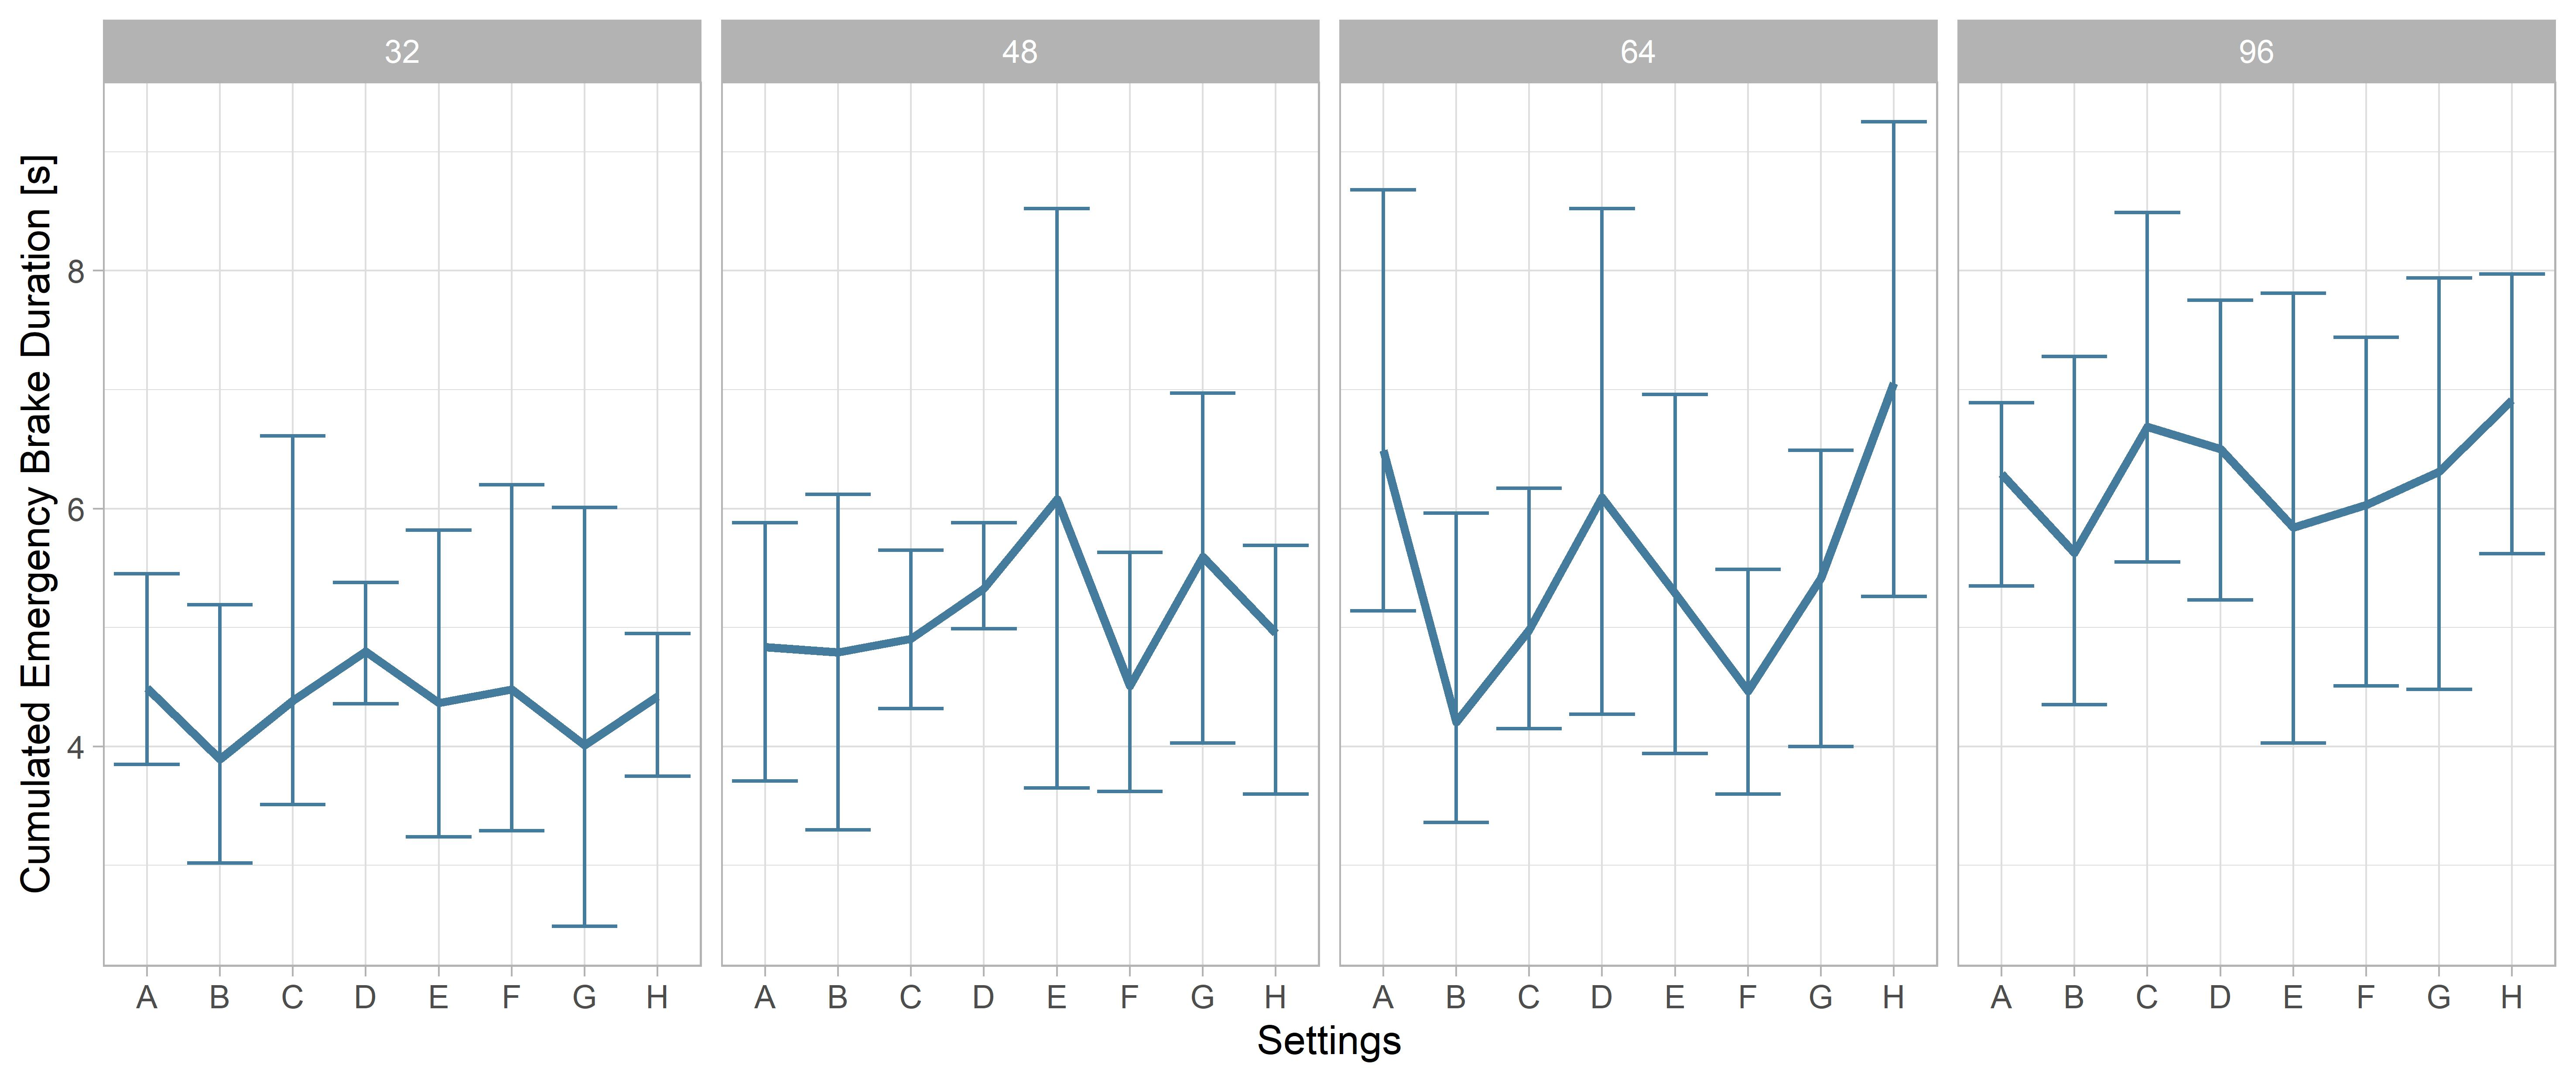
\includegraphics[width=1\linewidth]{simulations/population/plots/comparison}
	\caption{mean and error bars per population size}
	\label{fig:hyperparameter_tuning:population_results}
\end{figure}

In Figure \ref{fig:hyperparameter_tuning:population_results}, the results per population are plotted. The line corresponds to the mean, while the error bars show the spread (min to max) of all 5 repetitions. A higher spread in the results can be seen when looking at the smaller population sizes. Considering these findings, a population size of 96 was chosen. While such a high value will result in a performance impact, it was deemed more important to keep the variation low.

\section{Design of Experiment}
\label{sect:hyperparameter_tuning:design_of_experiment}
This section aims to find optimal settings for the remaining control parameters of the given problem. Following the conclusion from the previous Section \ref{sect:hyperparameter_tuning:population}, a population size of 96 will be fixated. In order to further tune the control parameter of the genetic algorithm, various different strategies can be used. Using automated approaches like 'grid search'~\cite{zahedi_search_2021} or 'simmulated annealing'~\cite{kirkpatrick_optimization_1983} might lead to good results with minimal effort. Grefenstette~\cite{grefenstette_optimization_1986} even suggests using a second, higher level genetic algorithm for the optimization process. The tuning of hyperparameter for these algorithms is however still needed. Due to performance considerations, many optimization methods did not fit the requirements. Executing one run for 30 generations takes around 3:50 hours. The high variance between runs requires a certain number of repetitions for each setting. Although two different workstations were available, the time required to execute the needed number of runs for these automated tests would exceed the available time budged. For this section, 8 repetitions were used per setting, which makes one evaluation last 30 hours.

A different approach is called design of experiment (DOE), also known as statistically designed experiments. DOE tries to find the cause and-effect relationship between the factors and the output of experiments. It uses factorial design where the variables in an experiment are named 'factors'. Each factor consists of at least two settings, with the actual number of settings being called 'levels'~\cite{yang_design_2009}. Design of experiment needs manual expertise to define which factors are possibly of importance and which settings each factor should have.

\begin{quote}
	\begin{em}
		\enquote{If the range of variable is too small, then we may miss lots of useful information. If the range is too large, then the extreme values might give infeasible experimental runs.}~\cite{yang_design_2009}
	\end{em}
\end{quote}

Subsequently, main effects and interactions can be calculated to find the best settings per factor. ANOVA (Analysis of Variance) will identify the significance of each factor and interaction. More details on these analysis tools will be provided in Section \ref{sect:hyperparameter_tuning:analysis_of_results}.

A full factorial design will test over all possible combinations of the selected factor levels. Looking at the proposed factors in Table \ref{tab:hyperparameter_tuning:settings_to_level}, 1024 runs\footnote{number of runs calculated using: \url{https://datatab.net/statistics-calculator/design-of-experiments}} are required, which is not feasible performance wise. A full factorial design has the drawback, that, as the number of factors k gets increased, the number of needed experimental runs increases exponentially, thus resulting in lengthy experiments. Yang and El-Haik~\cite{yang_design_2009} state that most of the results obtained by testing over all combinations are only used for estimating higher-order interactions, which are in most cases insignificant.

\subsection{Taguchi Method}
Various improvements to design of experiment have been but forward by Dr. Genichi Taguchi, such as reducing the influence of uncontrollable (noise) factors on processes and products as well as reducing variability~\cite{roy_primer_1990}. This master's thesis will not discuss all of Taguchi's proposed considerations; for more detail Roy~\cite{roy_primer_1990} as well as Yang and El-Haik~\cite{yang_design_2009} are recommended. Taguchi's proposed design of experiment is a fractional factorial design, which requires significantly fewer runs. In fractional factorial designs, only a fraction of all possible combinations is investigated~\cite{roy_primer_1990}. While different fractional factorial designs are available, Taguchi was chosen, because he provides a simple and easy-to-follow procedure that requires only a minimal number of runs. 

\begin{quote}
	\begin{em}
		\enquote{There are many similarities between “regular” experimental design and Taguchi's experimental design. However, in a Taguchi experiment, only the main effects and two-factor interactions are considered. Higher-order interactions are assumed to be non-existent. In addition, experimenters are asked to identify which interactions might be significant before conducting the experiment, through their knowledge of the subject matter.}~\cite{yang_design_2009}
	\end{em}
\end{quote}

Taguchi predefined a number of different orthogonal arrays where each row contains the specific levels (i.e the settings) of one experiment, while the columns correspond to the factors. The researcher has the responsibility to select an array based on the individual needs~\cite{li_taguchi_2021}. Using these orthogonal arrays instead of full factorial experiments will lead to a much smaller amount of simulation runs, while the full factorial experiments \enquote{might not provide appreciably more useful information}~\cite{roy_primer_1990}.

A big drawback of using Taguchi orthogonal arrays is the inability of evaluating higher-order interaction effects. Not only are these interaction effects impossible to evaluate, but they also have a negative influence on the performance. Orthogonal array experiments perform best in cases of minimal interaction between factors. While there is still a good chance of identifying the optimum condition, especially the performance estimate can be significantly off~\cite{roy_primer_1990}. Although Yang and El-Haik~\cite{yang_design_2009} state that in many cases higher-order interaction effects in factorial designs are seldom significant, this might not be the case for genetic algorithms. For example, according to \cite{kacprzyk_parameter_2007}, control parameters of a genetic algorithm \enquote{interact in highly non-linear ways.} If the proposed method is able to provide a suitable set of hyperparameter settings will be evaluated in Chapter \ref{chap:evaluation}.

\paragraph{Selection of an Orthogonal Array}
When choosing a suitable Taguchi orthogonal array, various factors have to be taken into account. According to Yang and El-Haik~\cite{yang_design_2009}, a three step procedure needs to be followed:

\begin{enumerate}
	\item Calculate the total degree of freedom (DOF). 
	\item Based on the following two rules, a standard orthogonal array should be selected:
	\begin{enumerate}
		\item The total DOF need to be smaller than the number of runs provided by the orthogonal array.
		\item All required factor level combinations need to be accommodated by the orthogonal array.
	\end{enumerate}
	
	\item Factors have to be assigned using these rules: 
	\begin{enumerate}
		\item In case the factor level does not fit into the orthogonal array, methods such as column merging and dummy levels can be used to modify the original array.
		\item Using the linear graph and interaction table, interactions can be defined. 
		\item In case some columns are not assigned, its possible to keep these columns empty.
	\end{enumerate}
\end{enumerate}

For this design of experiment, seven factors (three 4-level factors and four 2-level factors) have been selected. The choice of factors and levels to choose was made based on experience gained on Section \ref{sect:hyperparameter_tuning:population}. In Table \ref{tab:hyperparameter_tuning:settings_to_level}, every factor with the corresponding levels is listed.

\begin{table}[ht]
	\centering
	\small
	\begin{tabular}{ l|c|cccc }
		\hline
		Factors & Code & Level 1 & Level 2 & Level 3 & Level 4\\
		\hline
		CrossoverType 		& A & one point & two point & uni$^*$ 0.1 & uni$^*$ 0.5\\
		CrossoverRate    	& B & 0.2 & 0.5 & 0.8 & 0.9\\
		MutationRate   		& C & 0.01 & 0.1 & 0.3 & 0.5\\
		ChromosomeType   	& D & Time & Time+NPC & - & -\\
		GeneType			& E & Int & Dict & - & -\\
		TournamentSize 		& F & 2 & 4 & - & -\\
		IndMutationRate		& G & 0.1 & 0.5 & - & -\\
		\hline
	\end{tabular}
\caption{control parameters (factors) with corresponding settings (levels) - ($^*$uniform)}
\label{tab:hyperparameter_tuning:settings_to_level}
\end{table}

As already stated, Taguchi allows to only test for predetermined two-factor interactions; evaluating higher-order factor interactions is not possible~\cite{yang_design_2009}. Analysing interactions comes at the cost of degrees of freedom. An interaction between ChromosomeType and GeneType might be of interest and will thus be chosen. In order to minimized the required degrees of freedom (and correspondingly the required number of experiment runs), no additional interactions will be analysed.

\subsection{Selection of a Suitable Standard Orthogonal Array}
\label{sect:hyperparameter_tuning:selection_orthogonal_array}
The total degree of freedom can be calculated using the rules provided by Yang and El-Haik~\cite{yang_design_2009}:

\begin{enumerate}
	\item 1 DOF is always used for the overall mean. 
	\item Each factor has a DOF of NumberOfLevels - 1.
	\item Two-factor interactions require a DOF of: $(n_{factor1} - 1)(n_{factor2} - 1)$ where $n$ = number of levels.
\end{enumerate}

This leads to the following calculation for the needed three 4-level factors and four 2-level factors as well as the interaction ChromosomeType-GeneType:

\begin{equation}
	\begin{split}
		DOF & = 1 + 3 * (4 - 1) + 4 * (2 - 1) + 1 * (2 - 1) * (2 - 1) \\
		& = 15
	\end{split}
	 \label{equ:hyperparam_tuning:DOF}
\end{equation}

A $L_{16}$ array seems suitable to accommodate the required 15 DOF, which can be seen in table \ref{tab:hyperparameter_tuning:L16_orhtogonal_array}.

\begin{table}[ht]
	\centering
	\begin{tabular}{ |c||c|c|c|c|c|c|c|c|c|c|c|c|c|c|c|  }
		\hline
		   & \multicolumn{15}{c|}{ $L_{16}(2^{15})$ } \\
		NO.& 1 & 2 & 3 & 4 & 5 & 6 & 7 & 8 & 9 & 10& 11& 12& 13& 14&15\\
		\hline
		1  & 1 & 1 & 1 & 1 & 1 & 1 & 1 & 1 & 1 & 1 & 1 & 1 & 1 & 1 & 1\\
		2  & 1 & 1 & 1 & 1 & 1 & 1 & 1 & 2 & 2 & 2 & 2 & 2 & 2 & 2 & 2\\
		3  & 1 & 1 & 1 & 2 & 2 & 2 & 2 & 1 & 1 & 1 & 1 & 2 & 2 & 2 & 2\\
		4  & 1 & 1 & 1 & 2 & 2 & 2 & 2 & 2 & 2 & 2 & 2 & 1 & 1 & 1 & 1\\
		5  & 1 & 2 & 1 & 1 & 1 & 2 & 2 & 1 & 1 & 2 & 2 & 1 & 1 & 2 & 2\\
		6  & 1 & 2 & 2 & 1 & 1 & 2 & 2 & 2 & 2 & 1 & 1 & 2 & 2 & 1 & 1\\
		7  & 1 & 2 & 2 & 2 & 2 & 1 & 1 & 1 & 1 & 2 & 2 & 2 & 2 & 1 & 1\\
		8  & 1 & 2 & 2 & 2 & 2 & 1 & 1 & 2 & 2 & 1 & 1 & 1 & 1 & 2 & 2\\
		9  & 2 & 1 & 2 & 1 & 2 & 1 & 2 & 1 & 2 & 1 & 2 & 1 & 2 & 1 & 2\\
		10 & 2 & 1 & 2 & 1 & 2 & 1 & 2 & 2 & 1 & 2 & 1 & 2 & 1 & 2 & 1\\
		11 & 2 & 1 & 2 & 2 & 1 & 2 & 1 & 1 & 2 & 1 & 2 & 2 & 1 & 2 & 1\\
		12 & 2 & 1 & 2 & 2 & 1 & 2 & 1 & 2 & 1 & 2 & 1 & 1 & 2 & 1 & 2\\
		13 & 2 & 2 & 1 & 1 & 2 & 2 & 1 & 1 & 2 & 2 & 1 & 1 & 2 & 2 & 1\\
		14 & 2 & 2 & 1 & 1 & 2 & 2 & 1 & 2 & 1 & 1 & 2 & 2 & 1 & 1 & 2\\
		15 & 2 & 2 & 1 & 2 & 1 & 1 & 2 & 1 & 2 & 2 & 1 & 2 & 1 & 1 & 2\\
		16 & 2 & 2 & 1 & 2 & 1 & 1 & 2 & 2 & 1 & 1 & 2 & 1 & 2 & 2 & 1\\
		\hline
	\end{tabular}
	\caption{ $L_{16}(2^{15})$ taguchi orthogonal array taken from Roy~\cite{roy_primer_1990}}
	\label{tab:hyperparameter_tuning:L16_orhtogonal_array}
\end{table}

The 4-level factors need additional space, which will be generated using column merging, while the interaction will need to be assigned as well.
Either an interaction table or linear graphs of the $L_{16}$ array can be used for both column merging and interaction assignment~\cite{danacioglu_taguchi_2005}. Both illustrate the interaction relationships in the orthogonal array~\cite{yang_design_2009}.
The linear graph is more straight forward and will be the selected approach. While there are multiple linear graphs for the $L_{16}$ array, Figure \ref{fig:hyperparameter_tuning:linear_graph} describes the graph which best fits the requirements from Table \ref{tab:hyperparameter_tuning:settings_to_level}. If no suitable graph is found, they can be modified using rules described by Danacıoğlu and Muluk~\cite{danacioglu_taguchi_2005}.

\begin{figure}[H]
	\centering
	\begin{tikzpicture}
		% Define 1 2 3
		\node (Node2) at (0,0) {2};
		\node (Middle12) at (0,1) {};
		\node (Eclipse12) at (-0.8,0) {};
		\node (Node1) at (0,2) {1};
		
		\draw (Node2) -- node[midway, right] {3} (Node1);
		
		
		% Define 4 8 12
		\node (Node8) at (2,0) {8};
		\node (Middle84) at (2,1) {};
		\node (Eclipse84) at (1.2,0) {};
		\node (Node4) at (2,2) {4};
		
		\draw (Node8) -- node[midway, right] {12} (Node4);
		
		% Define 5 15 10
		\node (Node10) at (4,0) {10};
		\node (Middle105) at (4,1) {};
		\node (Eclipse105) at (3.2,0) {};
		\node (Node5) at (4,2) {5};
		
		\draw (Node10) -- node[midway, right] {15} (Node5);
		
		% Define 7 9 14
		\node (Node9) at (6,0) {9};
		\node (Node7) at (6,2) {7};
		
		\draw (Node9) -- node[midway, right] {14} (Node7);
		
		% Define 6 11 13
		\node (Node11) at (8,0) {11};
		\node (Node6) at (8,2) {6};
		
		\draw (Node11) -- node[midway, right] {13} (Node6);
	\end{tikzpicture}
	\caption{linear graph of $L_{16}(2^{15})$ taken from Yang and El-Haik~\cite{yang_design_2009}}
	\label{fig:hyperparameter_tuning:linear_graph}
\end{figure}

In a Taguchi linear graph, both nodes and connections represent columns in the orthogonal array. The interaction between two nodes is described by the connecting line~\cite{taguchi_taguchis_2005}. This is useful for both analysing interactions between columns as well as combining (merging) interacting columns in case a higher factor is needed.

\paragraph{Column Merging}
A, B and C are 4-level factors. The currently selected orthogonal array only fits 2-level factors. Through column merging, it is possible to extend columns to accommodate higher-order levels. As calculated in Equation \ref{equ:hyperparam_tuning:DOF}, a 4-level column requires three degrees of freedom, thus three 2-level columns need to be merged. Column merging needs the to-be-merged columns to be part of an interaction group~\cite{yang_design_2009}. The available interaction groups are visualized by the linear graph in Figure \ref{fig:hyperparameter_tuning:linear_graph}. Three 2-level interaction columns need to be selected first. One column is discarded and the remain two columns are merged using the rules in Table \ref{tab:hyperparameter_tuning:merging_rules}.

\begin{table}[ht]
	\centering
	\begin{tabular}{ |ccccccc|  }
		\hline
		\multicolumn{3}{|c}{ OLD COLUMN } & & & & NEW COLUMN \\
		\hline
		& 1 & 1 & & -> & & 1\\
		& 1 & 2 & & -> & & 2\\
		& 2 & 1 & & -> & & 3\\
		& 2 & 2 & & -> & & 4\\
		\hline
	\end{tabular}
	\caption{merging rules taken from Roy~\cite{roy_primer_1990}}
	\label{tab:hyperparameter_tuning:merging_rules}
\end{table}

The 4-level factor can then be assigned to this newly generated column. Because three 4-level factors are needed for the current experiment, a total of nine 2-level columns have to be merged.

\paragraph{Assigning Interactions}
The interaction between both 2-level factors is also assigned by utilizing the linear graph. An interaction between ChromosomeType and GeneType seems possible, thus D and E will be assigned to connected nodes in the linear graph. The resulting graph can be seen in Figure \ref{fig:hyperparameter_tuning:linear_graph_assigned}. An interaction between F and G can not be investigated, as the chosen orthogonal array is not able to fit the additional 1 degree of freedom (see Equation \ref{equ:hyperparam_tuning:DOF}).

\begin{figure}[H]
	\centering
	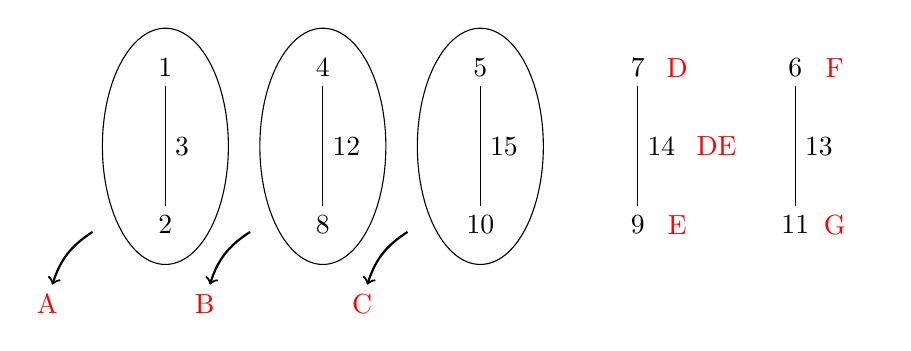
\begin{tikzpicture}
		% Define 1 2 3
		\node (Node2) at (0,0) {2};
		\node (Middle12) at (0,1) {};
		\node (Eclipse12) at (-0.8,0) {};
		\node (Node1) at (0,2) {1};
		\node[red] (A) at (-1.5, -1) {A};
	
		\draw (Node2) -- node[midway, right] {3} (Node1);
		\draw (Middle12) ellipse (0.8cm and 1.5cm);
		\draw[->, thick] (Eclipse12) to[bend right=20] (A);
		
		
		% Define 4 8 12
		\node (Node8) at (2,0) {8};
		\node (Middle84) at (2,1) {};
		\node (Eclipse84) at (1.2,0) {};
		\node (Node4) at (2,2) {4};
		\node[red] (B) at (0.5, -1) {B};
		
		\draw (Node8) -- node[midway, right] {12} (Node4);
		\draw (Middle84) ellipse (0.8cm and 1.5cm);
		\draw[->, thick] (Eclipse84) to[bend right=20] (B);
		
		% Define 5 15 10
		\node (Node10) at (4,0) {10};
		\node (Middle105) at (4,1) {};
		\node (Eclipse105) at (3.2,0) {};
		\node (Node5) at (4,2) {5};
		\node[red] (C) at (2.5, -1) {C};
		
		\draw (Node10) -- node[midway, right] {15} (Node5);
		\draw (Middle105) ellipse (0.8cm and 1.5cm);
		\draw[->, thick] (Eclipse105) to[bend right=20] (C);
		
		% Define 7 9 14
		\node (Node9) at (6,0) {9};
		\node (Node7) at (6,2) {7};
		\node[red] (E) at (6.5,0) {E};
		\node[red] (D) at (6.5,2) {D};
		\node[red] (DE) at (7,1) {DE};
		
		\draw (Node9) -- node[midway, right] {14} (Node7);
		
		
		% Define 6 11 13
		\node (Node11) at (8,0) {11};
		\node (Node6) at (8,2) {6};
		\node[red] (G) at (8.5,0) {G};
		\node[red] (F) at (8.5,2) {F};
		\node (FG) at (9,1) {};
		
		\draw (Node11) -- node[midway, right] {13} (Node6);
	\end{tikzpicture}
\caption{modified linear graph}
\label{fig:hyperparameter_tuning:linear_graph_assigned}
\end{figure}

Combining columns 1 2 3 to A, 4 8 12 to B and 5 10 15 to C using rules defined by Table \ref{tab:hyperparameter_tuning:merging_rules} is done in Table \ref{tab:hyperparameter_tuning:merging_columns}. Removing the old and inserting the new columns in the table and transcoding 7 to D, 9 to E, 14 to DE, 6 to F and 11 to G results in the final Table \ref{tab:hyperparameter_tuning:final_taguchi}.

\begin{table}[ht]
	\centering
	\begin{tabular}{ |c||cccc|cccc|cccc|  }
		\hline
		NO.& 1 & 2 & & \sout{3} & 4 & 8 & &  \sout{12} & 5 & 10 & &  \sout{15}\\
		\hline
		1  & \multicolumn{4}{c}{\sout{1 1} > 1 } & \multicolumn{4}{|c|}{\sout{1 1} > 1 } & \multicolumn{4}{c|}{\sout{1 1} > 1 }\\
		2  & \multicolumn{4}{c}{\sout{1 1} > 1 } & \multicolumn{4}{|c|}{\sout{1 2} > 2 } & \multicolumn{4}{c|}{\sout{1 2} > 2 }\\
		3  & \multicolumn{4}{c}{\sout{1 1} > 1 } & \multicolumn{4}{|c|}{\sout{2 1} > 3 } & \multicolumn{4}{c|}{\sout{2 1} > 3 }\\
		4  & \multicolumn{4}{c}{\sout{1 1} > 1 } & \multicolumn{4}{|c|}{\sout{2 2} > 4 } & \multicolumn{4}{c|}{\sout{2 2} > 4 }\\
		5  & \multicolumn{4}{c}{\sout{1 2} > 2 } & \multicolumn{4}{|c|}{\sout{1 1} > 1 } & \multicolumn{4}{c|}{\sout{1 2} > 2 }\\
		6  & \multicolumn{4}{c}{\sout{1 2} > 2 } & \multicolumn{4}{|c|}{\sout{1 2} > 2 } & \multicolumn{4}{c|}{\sout{1 1} > 1 }\\
		7  & \multicolumn{4}{c}{\sout{1 2} > 2 } & \multicolumn{4}{|c|}{\sout{2 1} > 3 } & \multicolumn{4}{c|}{\sout{2 2} > 4 }\\
		8  & \multicolumn{4}{c}{\sout{1 2} > 2 } & \multicolumn{4}{|c|}{\sout{2 2} > 4 } & \multicolumn{4}{c|}{\sout{2 1} > 3 }\\
		9  & \multicolumn{4}{c}{\sout{2 1} > 3 } & \multicolumn{4}{|c|}{\sout{1 1} > 1 } & \multicolumn{4}{c|}{\sout{2 1} > 3 }\\
		10 & \multicolumn{4}{c}{\sout{2 1} > 3 } & \multicolumn{4}{|c|}{\sout{1 2} > 2 } & \multicolumn{4}{c|}{\sout{2 2} > 4 }\\
		11 & \multicolumn{4}{c}{\sout{2 1} > 3 } & \multicolumn{4}{|c|}{\sout{2 1} > 3 } & \multicolumn{4}{c|}{\sout{1 1} > 1 }\\
		12 & \multicolumn{4}{c}{\sout{2 2} > 3 } & \multicolumn{4}{|c|}{\sout{2 2} > 4 } & \multicolumn{4}{c|}{\sout{1 2} > 2 }\\
		13 & \multicolumn{4}{c}{\sout{2 2} > 4 } & \multicolumn{4}{|c|}{\sout{1 1} > 1 } & \multicolumn{4}{c|}{\sout{2 2} > 4 }\\
		14 & \multicolumn{4}{c}{\sout{2 2} > 4 } & \multicolumn{4}{|c|}{\sout{1 2} > 2 } & \multicolumn{4}{c|}{\sout{2 1} > 3 }\\
		15 & \multicolumn{4}{c}{\sout{2 2} > 4 } & \multicolumn{4}{|c|}{\sout{2 1} > 3 } & \multicolumn{4}{c|}{\sout{1 2} > 2 }\\
		16 & \multicolumn{4}{c}{\sout{2 2} > 4 } & \multicolumn{4}{|c|}{\sout{2 2} > 4 } & \multicolumn{4}{c|}{\sout{1 1} > 1 }\\
		\hline
	\end{tabular}
	\caption{Building 4 Level columns from 2 Level columns}
	\label{tab:hyperparameter_tuning:merging_columns}
\end{table}

\begin{table}[ht]
	\centering
	\begin{tabular}{ |c||c|c|c|c|c|c|c|c|  }
		\hline
		NO.& A & B & C & D & E & F & G & DE\\
		\hline
		1  & 1 & 1 & 1 & 1 & 1 & 1 & 1 & 1\\
		2  & 1 & 2 & 2 & 1 & 2 & 1 & 2 & 2\\
		3  & 1 & 3 & 3 & 2 & 1 & 2 & 1 & 2\\
		4  & 1 & 4 & 4 & 2 & 2 & 2 & 2 & 1\\
		5  & 2 & 1 & 2 & 2 & 1 & 2 & 2 & 2\\
		6  & 2 & 2 & 1 & 2 & 2 & 2 & 1 & 1\\
		7  & 2 & 3 & 4 & 1 & 1 & 1 & 2 & 1\\
		8  & 2 & 4 & 3 & 1 & 2 & 1 & 1 & 2\\
		9  & 3 & 1 & 3 & 2 & 2 & 1 & 2 & 1\\
		10 & 3 & 2 & 4 & 2 & 1 & 1 & 1 & 2\\
		11 & 3 & 3 & 1 & 1 & 2 & 2 & 2 & 2\\
		12 & 3 & 4 & 2 & 1 & 1 & 2 & 1 & 1\\
		13 & 4 & 1 & 4 & 1 & 2 & 2 & 1 & 2\\
		14 & 4 & 2 & 3 & 1 & 1 & 2 & 2 & 1\\
		15 & 4 & 3 & 2 & 2 & 2 & 1 & 1 & 1\\
		16 & 4 & 4 & 1 & 2 & 1 & 1 & 2 & 2\\
		\hline
	\end{tabular}
	\caption{final version of orthogonal array}
	\label{tab:hyperparameter_tuning:final_taguchi}
\end{table}


\subsection{Result Analysis}
\label{sect:hyperparameter_tuning:analysis_of_results}
Table \ref{tab:hyperparameter_tuning:final_taguchi} will provide the settings for all needed test runs (the interaction column DE can be ignored until the evaluation). Transcoding all factors and levels to get the corresponding setting is done in Table \ref{tab:hyperparameter_tuning:settings_to_level}. Every setting will be repeated 8 times to reduce randomness and gain information about variance. Running the genetic algorithm with these 16 different settings each repeated 8 times took 10 days on the two workstations described in Section \ref{sect:hyperparameter_tuning:simulation_setup}. The results are found in the Appendix at Table \ref{tab:appendix:hyperparameter_tuning_final_taguchi}.

\subsubsection{ANOVA}
ANOVA analysis (analysis of variance) will provide information on the magnitude of contribution of the main effects and interactions. The calculation of ANOVA on a Taguchi experiment is the same as for a classical design of experiment~\cite{yang_design_2009}. Calculating ANOVA was done with the programming language R\footnote{\href{https://www.r-project.org/}{https://www.r-project.org/}} and the result can be seen in Table \ref{tab:taguchi:anova_results}.

\begin{table}[ht]
	\centering
	\begin{tabular}{lrrrrr}
		\hline
		& Df & Sum Sq & Mean Sq & F value & Pr($>$F) \\ 
		\hline
		A & 3 & 23.89 & 7.96 & 6.59 & 0.0004 \\ 
		B & 3 & 5.00 & 1.67 & 1.38 & 0.2532 \\ 
		C & 3 & 34.32 & 11.44 & 9.46 & 0.0000 \\ 
		D & 1 & 3.88 & 3.88 & 3.21 & 0.0759 \\ 
		E & 1 & 0.35 & 0.35 & 0.29 & 0.5912 \\ 
		F & 1 & 18.91 & 18.91 & 15.64 & 0.0001 \\ 
		G & 1 & 6.98 & 6.98 & 5.77 & 0.0179 \\ 
		D:E & 1 & 4.10 & 4.10 & 3.40 & 0.0680 \\ 
		Residuals & 113 & 136.60 & 1.21 &  &  \\ 
		\hline
	\end{tabular}
	\caption{ANOVA results}
	\label{tab:taguchi:anova_results}
\end{table}

The sum of squares column tells how much of the total variation is explained by the model. The variance is broken down into the factors A-G along with the interaction D:E. The residual sum of squares shows the difference between the model's prediction versus what was actually observed (i.e the variance that can not be explained by the model)~\cite{field_discovering_2012}. The F ratio (or value) measures the ratio of variance explained by the factor and the variation explained by the error term~\cite{field_discovering_2012}. Simply speaking, how good is the model versus how bad is the model. Finally, the p-value (in column labelled Pr(>F)) shows how likely the size of the given F ratio is obtained in case there is no effect on the results. Commonly, if p is smaller than 0.05, the effect can be viewed as statistically significant~\cite{field_discovering_2012}. The number of DOF is a result from the number of repetitions and can be calculated with the Equation \ref{equ:hyperparam_tuning:full_DOF} (taken from Roy~\cite{roy_primer_1990}).

\begin{equation}
	\begin{split}
		DOF & = totalNumberOfResults - 1 \\
		& = numberOfTrials * numberOfRepetitions - 1 \\
		& = 16 * 8 - 1 = 127
	\end{split}
	\label{equ:hyperparam_tuning:full_DOF}
\end{equation}

The multiple R-squared value of the model is 0.416 while the adjusted R-squared value is 0.344. Multiple R-squared gives a measure on how much variability in the outcome is explained by the predictors~\cite{field_discovering_2012}. Having only 41.6\% does not seem optimal. Field et al.~\cite{field_discovering_2012} state further that a model which generalizes well has an adjusted R-squared value that is similar to multiple R-squared, which is also not the case. The high error might possibly be explained by the huge search space in the scenario. Increasing the population and number of generations can lead to improvements, however at the cost of computational time. Whether the model, having this much of an error, will perform well compared to either a genetic algorithm build from values from the literature or compared to random search will be evaluated in Section \ref{chap:evaluation}.

Looking at the factors as well as the interaction, significant factors can be seen. The highest F value has the factor F (TournamentSize). The factor is significant with F(1, 112) = 15.64, p < 0.001. Next, the C (MutationRate) is significant with F(3, 112) = 9.46, p < 0.001. A (CrossoverType) is also significant F(3, 112) = 6.59, p < 0.001. Finally G (IndependendMutationRate) is significant with F(1, 112) = 5.77, p < 0.05. D (ChromosomeType) and the interaction D:E will be mentioned as well with F(1, 112) = 3.21, p < 0.1 and F(1, 112) = 3.4, p < 0.1 respectively. There is not enough evidence to suggest significance for the factors B (CrossoverRate) and E (GeneType). Particularly noteworthy is the insignificance of the CrossoverRate. The low influence of GeneType, however, might be explained by the fact, that it does not have an impact on the action selected apart from more granularity of the parameters when Dictionary encoding is used. To calculate the percentage contribution of each factor, Equations \ref{equ:hyperparam_tuning:ss_t} and \ref{equ:hyperparam_tuning:contribution} (gathered from from Yang and El-Haik~\cite{yang_design_2009}) are used.

\begin{equation}
	\begin{split}
		SS_T & = SS_A + SS_B + SS_C + ... + SS_{error}
	\end{split}
	 \label{equ:hyperparam_tuning:ss_t}
\end{equation}

\begin{equation}
	\begin{split}
		contribution_A = SS_A / SS_T * 100
	\end{split}
	 \label{equ:hyperparam_tuning:contribution}
\end{equation}

The percentage contribution of all factors is plotted in \ref{fig:hyperparam_tuning:percentage_contribution} and again shows the high error of the model. 

\begin{figure}[ht] 
	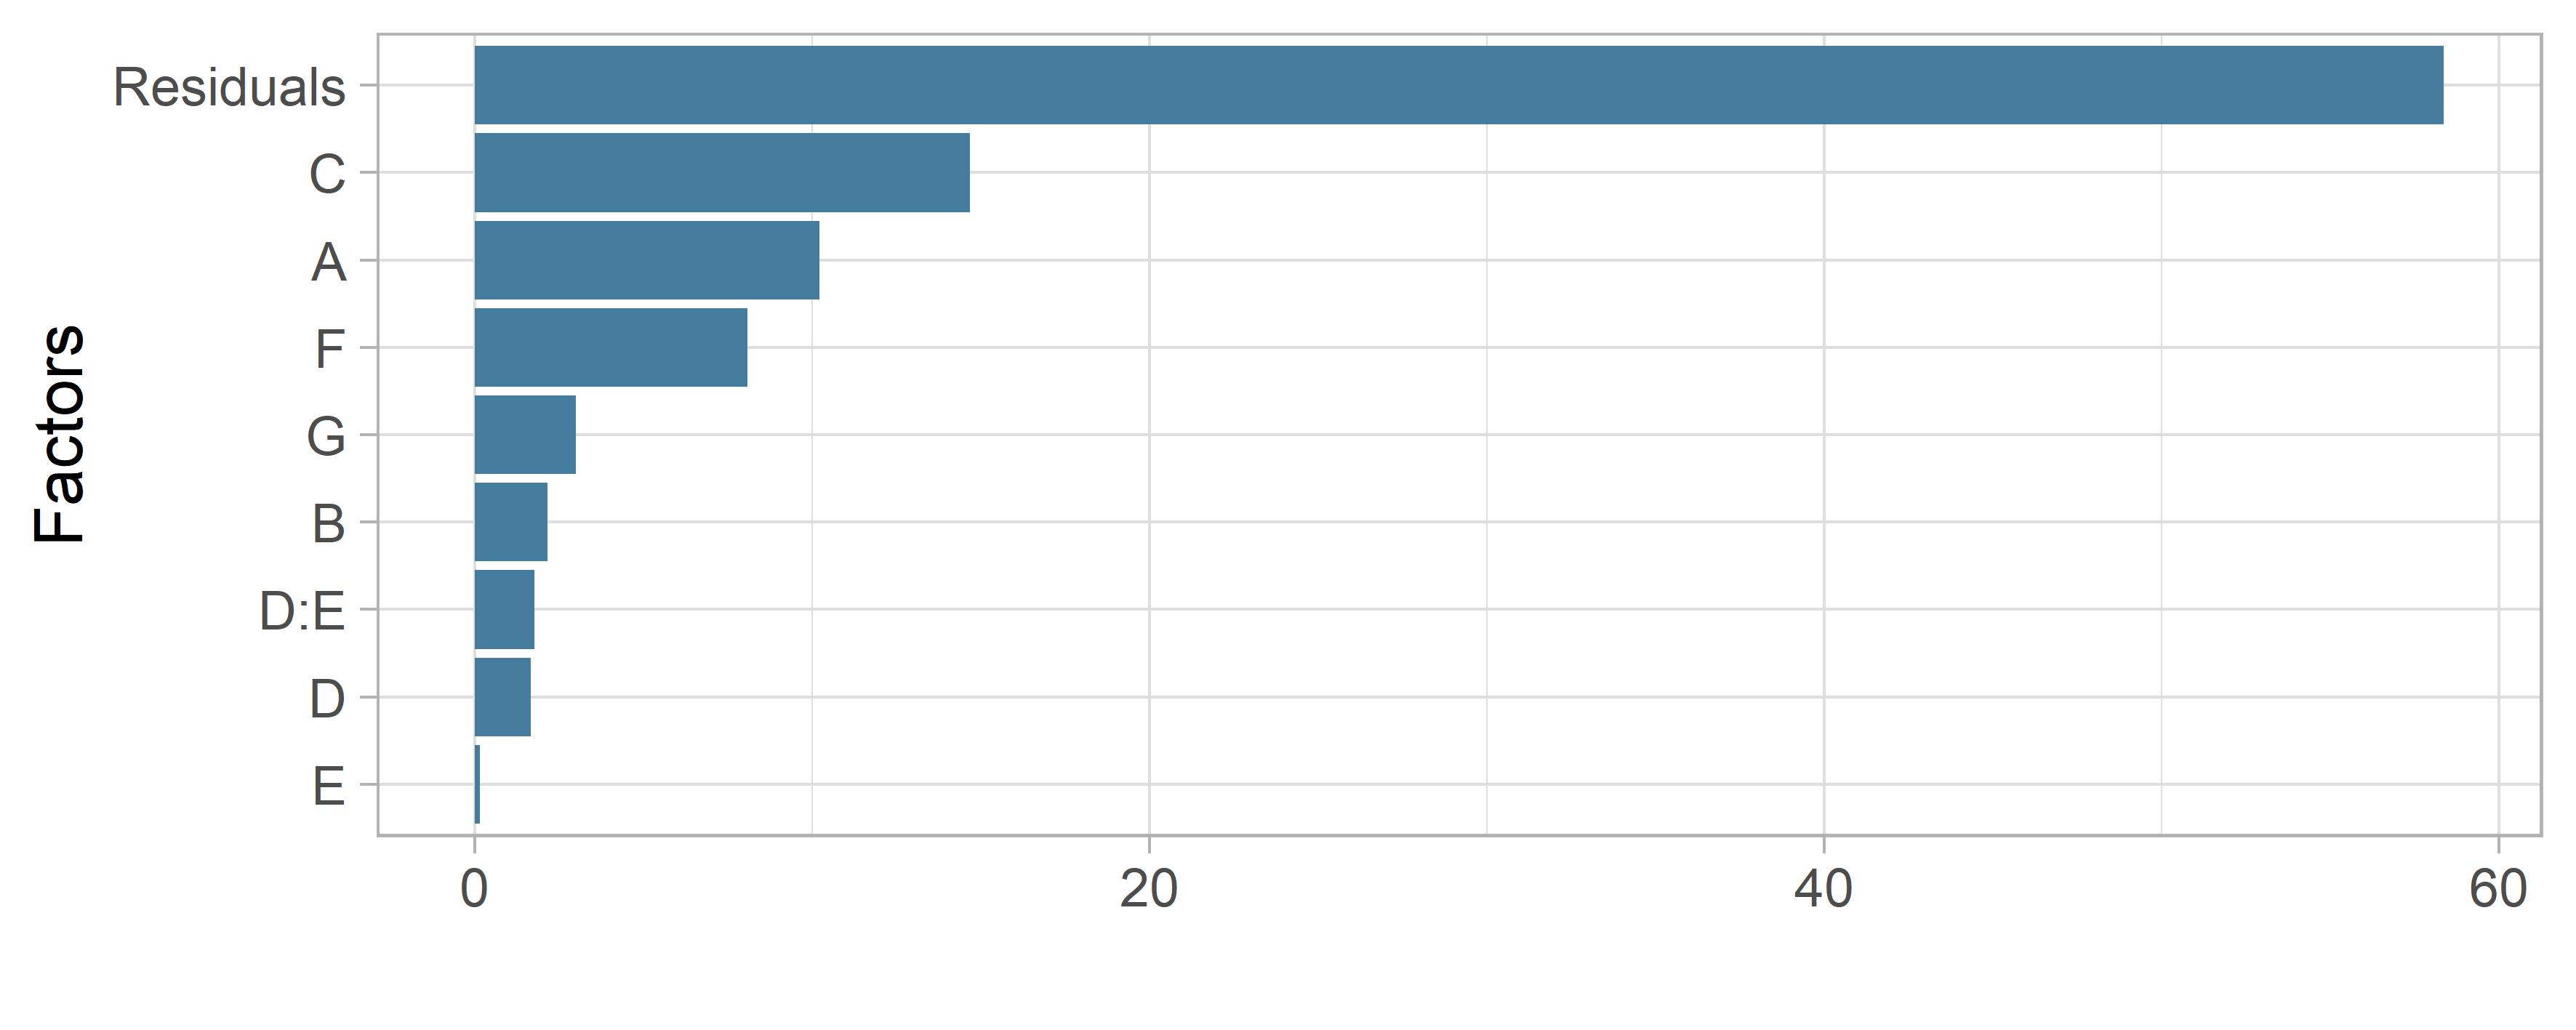
\includegraphics[width=1\linewidth]{simulations/taguchi/plots/percentage_contribution}
	\caption{percentage contribution}
	\label{fig:hyperparam_tuning:percentage_contribution}
\end{figure}

\subsubsection{Main-effects and interaction chart}
Identifying the optimal conditions needs analysis of the main effects per factor. They allow to predict the levels that lead to the best result~\cite{roy_primer_1990}.

\begin{quote}
	\begin{em}
		\enquote{The main-effects chart is a plot of average responses at different levels of a factor versus the factor levels.}~\cite{yang_design_2009}
	\end{em}
\end{quote}

For every factor, the mean of all results per level is summed up and subsequently divided by the number of runs per level. The resulting main-effect charts are visualized in Figure \ref{fig:hyperparam_tuning:main_effects}. In case there is no interaction, the optimal setting is easily determined by using the main effects chart. Go over every factor in the chart and use the best level (in this experiment, the level with the highest value).

\begin{figure}[ht] 
	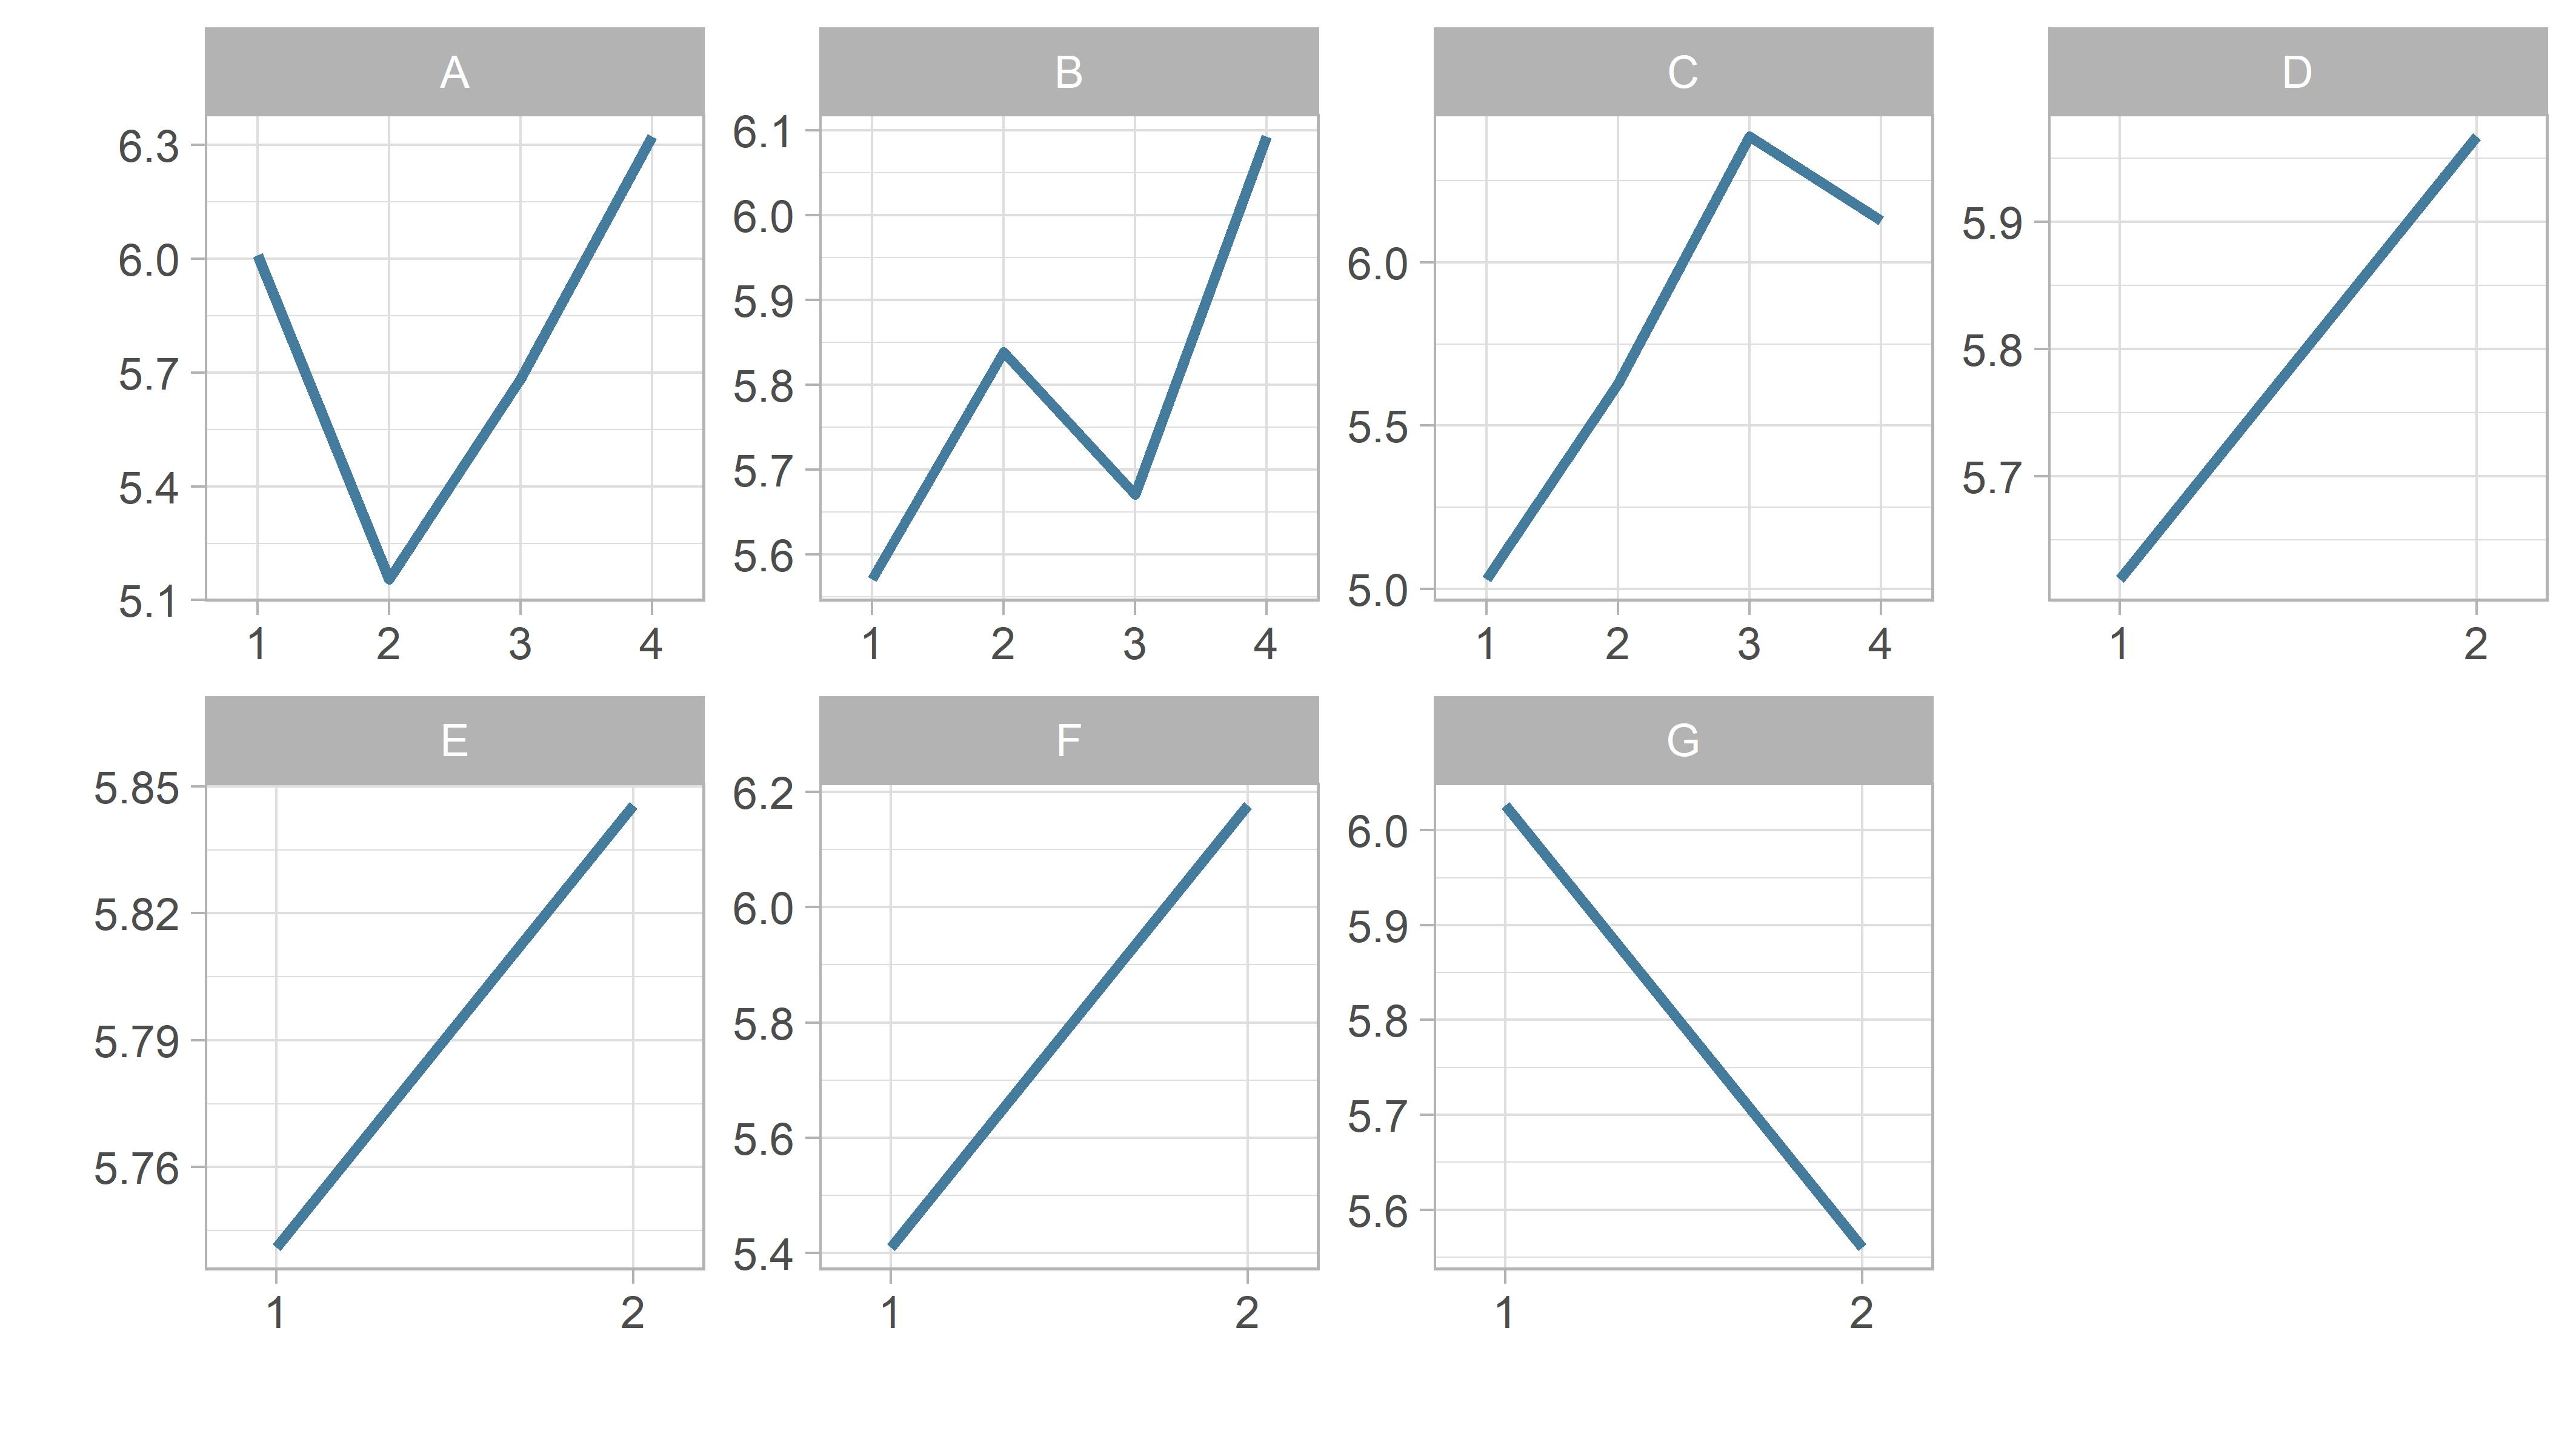
\includegraphics[width=1\linewidth]{simulations/taguchi/plots/main_effects}
	\caption{Main Effects}
	\label{fig:hyperparam_tuning:main_effects}
\end{figure}


 If interactions, however, exist, they might have an influence on the best settings and need further investigation~\cite{yang_design_2009}. The previously defined interaction is visualized in an interaction plot in Figure \ref{fig:hyperparam_tuning:interaction_plot}. The calculation is similar to calculating main effects, now the mean response for each level combination is summed up and divided by the number of runs per combination. The crossing of lines in the interaction plot indicates that an interaction between the two factors might exist~\cite{field_discovering_2012}. The more parallel the lines are, the less likely an interaction. The magnitude of the angle between the lines corresponds to the degree of interaction presence~\cite{roy_primer_1990}.

\begin{figure}[ht] 
	\centering
	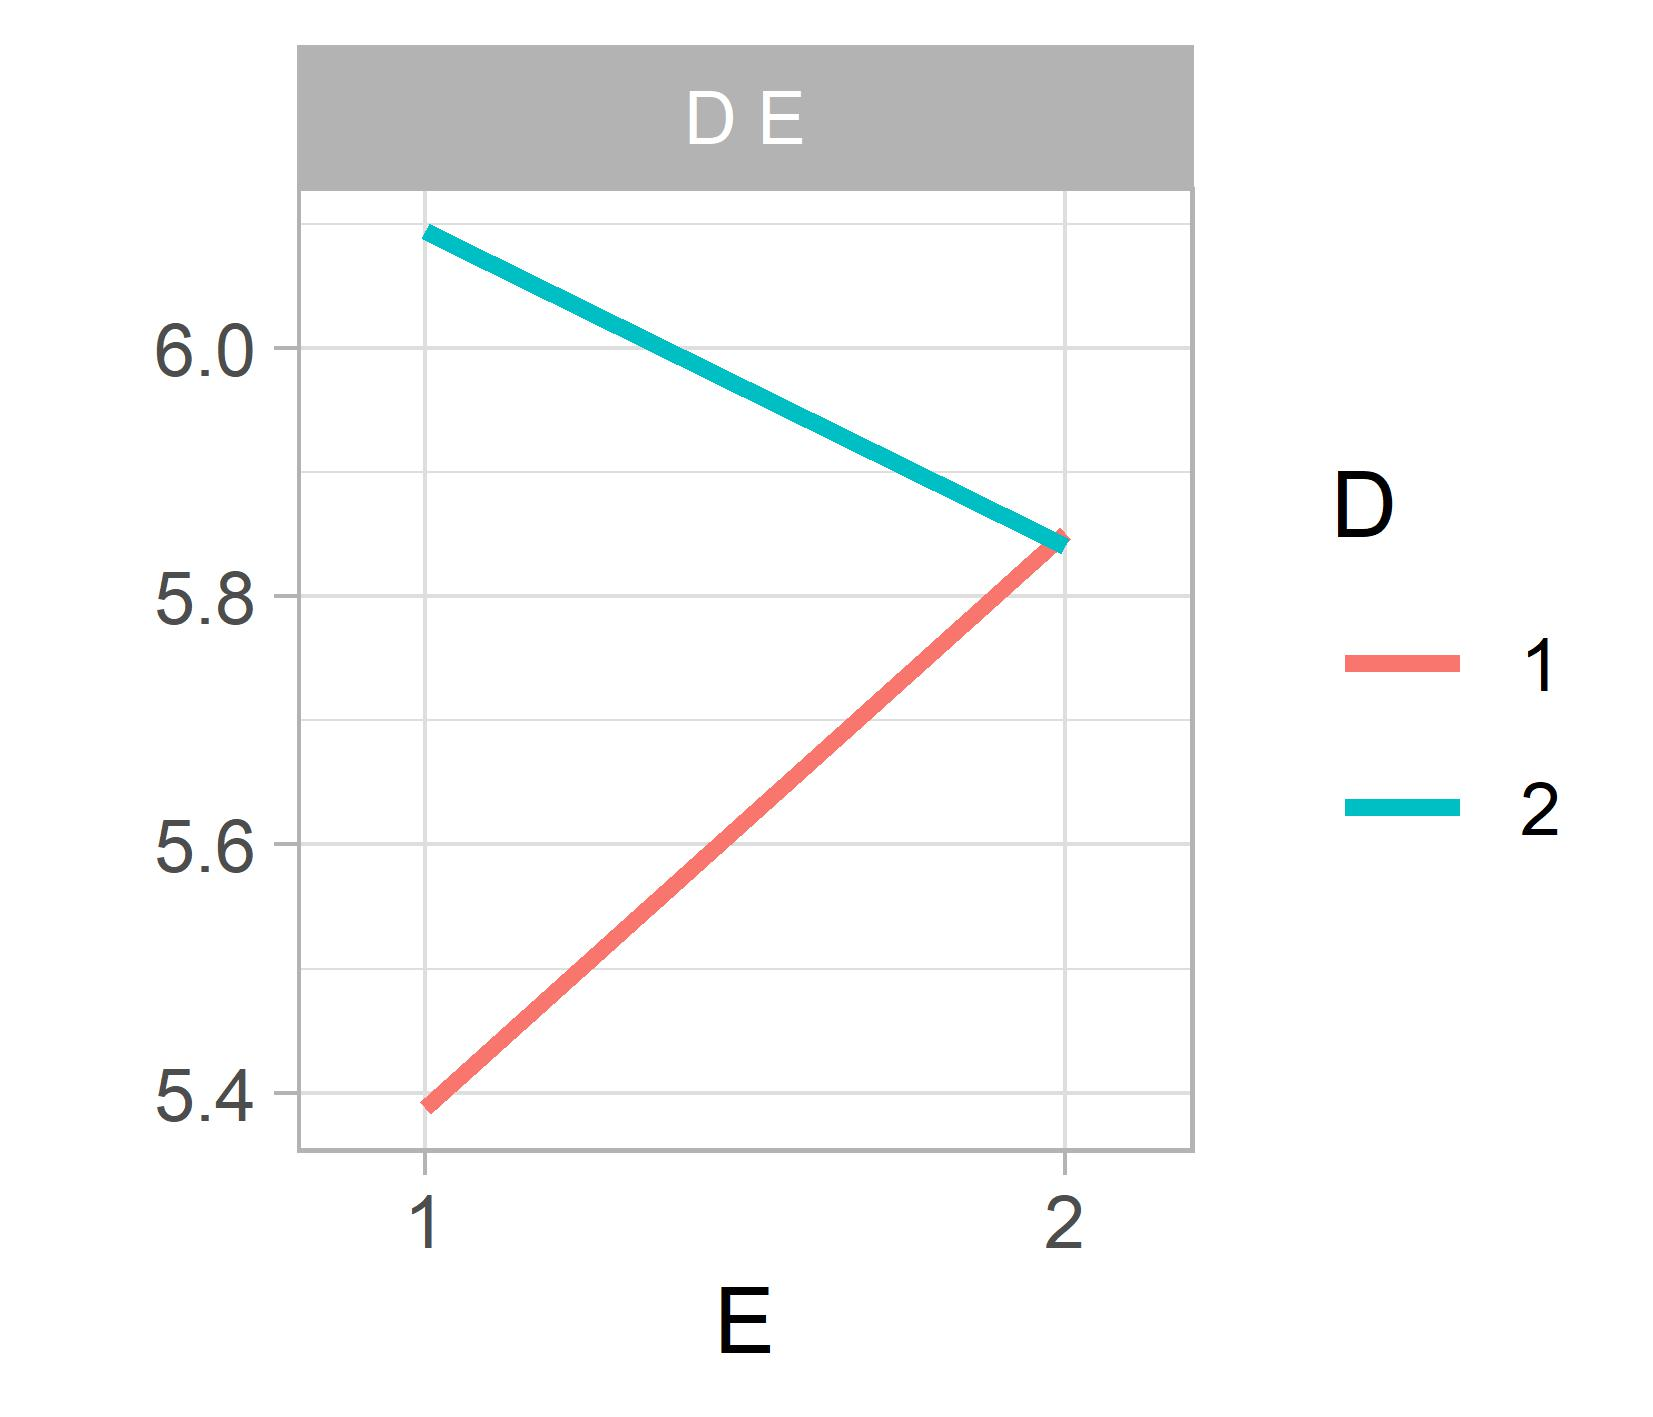
\includegraphics[width=0.4\linewidth]{simulations/taguchi/plots/test_of_interaction}
	\caption{interaction plot}
	\label{fig:hyperparam_tuning:interaction_plot}
\end{figure}

\subsubsection{Selection of optimal setting}
When choosing the optimal setting, the first step is to look at the best main effects combination. For this experiment, the best combination according the main effects is the following: $A_4$, $B_4$, $C_3$, $D_2$, $E_2$, $F_2$, $G_1$.

Analysing the interaction graph and the ANOVA table, the interaction D:E however might be significant. The interaction plot in Figure \ref{fig:hyperparam_tuning:interaction_plot} suggest $D_2$ and $E_1$ as the best combination. This is optimal, as $D_2$ is also recommended by the main effects. While $E_1$ does not correspond to its main effect, the low F value of the factor E suggests low significance anyway. Concluding this line of thought, the combination $A_4$, $B_4$, $C_3$, $D_2$, $E_1$, $F_2$, $G_1$ is preferred.

\paragraph{Optimum performance calculation}
\label{sect:hyperparameter_tuning:optimum_perf_caluclation}
To calculate the predicted results of a genetic algorithm with these settings, optimal performance calculation can be applied. Equation \ref{equ:hyperparameter_tuning:optimum_perf_main_effect}, which incorporates only the suggested main effects, and Equation \ref{equ:hyperparameter_tuning:optimum_perf_included_interaction}, which includes the additional interaction term D:E. The calculation formulas are sourced from Roy~\cite{roy_primer_1990}.

\begin{equation}
	\begin{split}
		Y_{opt} &= \overline{T} + (\overline{A_4} - \overline{T}) + (\overline{B_4} - \overline{T}) + (\overline{C_3} - \overline{T}) + (\overline{D_2} - \overline{T}) + \\& (\overline{E_2} - \overline{T}) + (\overline{F_2} - \overline{T}) + (\overline{G_1} - \overline{T}) \\
			&= 8.06
	\end{split}
	 \label{equ:hyperparameter_tuning:optimum_perf_main_effect}
\end{equation}


\begin{equation}
	\begin{split}
		Y_{opt} &= \overline{T} + (\overline{A_4} - \overline{T}) + (\overline{B_4} - \overline{T}) + (\overline{C_3} - \overline{T}) + (\overline{D_2} - \overline{T}) + \\& (\overline{E_1} - \overline{T})  + ([\overline{DxE}]_2 - \overline{T})  + (\overline{F_2} - \overline{T}) + (\overline{G_1} - \overline{T}) \\
		&= 8.13
	\end{split}
	 \label{equ:hyperparameter_tuning:optimum_perf_included_interaction}
\end{equation}

The inclusion of the interaction term D:E results in an improved performance estimation from 8.06 to 8.13. Consequently, the final optimal combination of control parameters is determined as follows: CrossoverType: Uniform 0.5, CrossoverRate: 0.9, MutationRate: 0.3, ChromosomeType: Time+NPC, GeneType: Integer, TournamentSize: 4 and IndividualMutationRate: 0.1.

The added higher granularity for the crossover function was preferred, which is provided by the chromosome encoding 'Time+NPC'. This encoding allows for the crossover operation to exchange actions between actors across different time steps. Notably, the choice of Uniform 0.5 as the CrossoverType as well as the high CrossoverRate and MutationRate is surprising. It remains to be seen, if the genetic algorithms will behave similar to random search or if the high rates will contribute to maintain diversity in its population.

\subsubsection{Signal-to-Noise Ratio}
As discussed earlier, the ANOVA model has a high error, which suggests high randomness. Taguchi recommends using signal-to-noise ratio (S/N) to reduce the variability, as using only the mean of the results (which is used when calculating the main effects) does not take the variation into account~\cite{roy_primer_1990}. S/N quantifies the ratio between the 'desired' signal to the 'undesired' noise. Essentially, a higher signal-to-noise ratio corresponds to reduced variance.

\begin{quote}
	\begin{em}
		\enquote{The use of the S/N ratio offers an objective way to look at the two characteristics (consistency and average value) together.}~\cite{roy_primer_1990}
	\end{em}
\end{quote}

S/N is calculated in two steps~\cite{roy_primer_1990}. The first step involves determining  the mean square deviation (MSD). Depending on the quality characteristic, a different equation has to be chosen. In this scenario, a higher result is better, thus Equation \ref{equ:hyperparam_tuning:MSD} is used for each repetition, with $y_1$ being the result of repetition 1 and $n$ the number of repetitions. The signal-to-noise ratio is calculated in the second step in Equation \ref{equ:hyperparam_tuning:S_N}.

\begin{equation}
	\begin{split}
		MSD & = (1/y^2_1 + 1/y^2_2 + 1/y^2_3 + ... ) / n
	\end{split}
	 \label{equ:hyperparam_tuning:MSD}
\end{equation}

\begin{equation}
	\begin{split}
		S/N & = -10 log_{10} (MSD)
	\end{split}
	 \label{equ:hyperparam_tuning:S_N}
\end{equation}

Generating the main effects and performing ANOVA is done using the S/N instead. As a side note, it's important to mention that only 15 DOF are available for the ANOVA analysis, as repetitions per run are merged when calculating S/N, which can be observed in Equation \ref{equ:hyperparam_tuning:S_N_anova_DOF}.

\begin{equation}
	\begin{split}
		DOF & = totalNumberOfResults - 1 \\
		& = numberOfTrials * 1 - 1 \\
		& = 16 - 1 = 15
	\end{split}
	 \label{equ:hyperparam_tuning:S_N_anova_DOF}
\end{equation}

\begin{table}[ht]
	\centering
	\begin{tabular}{lrrrrr}
		\hline
		& Df & Sum Sq & Mean Sq & F value & Pr($>$F) \\ 
		\hline
		A & 3 & 5.14 & 1.71 & 3.54 & 0.3682 \\ 
		B & 3 & 2.04 & 0.68 & 1.40 & 0.5397 \\ 
		C & 3 & 10.59 & 3.53 & 7.28 & 0.2644 \\ 
		D & 1 & 1.29 & 1.29 & 2.67 & 0.3498 \\ 
		E & 1 & 0.39 & 0.39 & 0.81 & 0.5329 \\ 
		F & 1 & 4.43 & 4.43 & 9.15 & 0.2033 \\ 
		G & 1 & 2.28 & 2.28 & 4.70 & 0.2751 \\ 
		D:E & 1 & 0.92 & 0.92 & 1.89 & 0.4005 \\ 
		Residuals & 1 & 0.48 & 0.48 &  &  \\ 
		\hline
	\end{tabular}
	\caption{S/N ANOVA results}
	\label{tab:hyperparameter_tuning:s_n_anova_results}
\end{table}

Based on the p values obtained from the ANOVA results in Table \ref{tab:hyperparameter_tuning:s_n_anova_results}, no factor is able to reject the null hypothesis, which states that a factor has no significant effect. Considering this fact, further investigations were deemed unnecessary. The often recommend signal-to-noise ratio does not appear suitable for this experiment, thus the previously calculated settings in Paragraph \ref{sect:hyperparameter_tuning:optimum_perf_caluclation} will remain unchanged.

\subsubsection{Elite Selection}
Although the optimal hyperparameter setting are reviewed in Chapter \ref{chap:evaluation}, a problem was obvious when analysing results of a GA using the settings from Section \ref{sect:hyperparameter_tuning:optimum_perf_caluclation}. Setbacks in the fitness value between two generations happen frequently, likely due to the high crossover and mutation rates. In order to mitigate this problem, elite selection with a size of 2 was implemented. Per generation, the two best individuals are now copied into the next generation without modifications, which makes worse performance between generations not possible. It is important to note, that these two individuals can still be selected by tournament selection for modification, its just that a copy of them is automatically saved. Figure \ref{fig:hyperparameter_tuning:elite_no_elite_comp} compares both no elite selection with an elite selection of 2. For a few selected repetitions, the best individual fitness per generation is plotted.

\begin{figure}[ht] 
	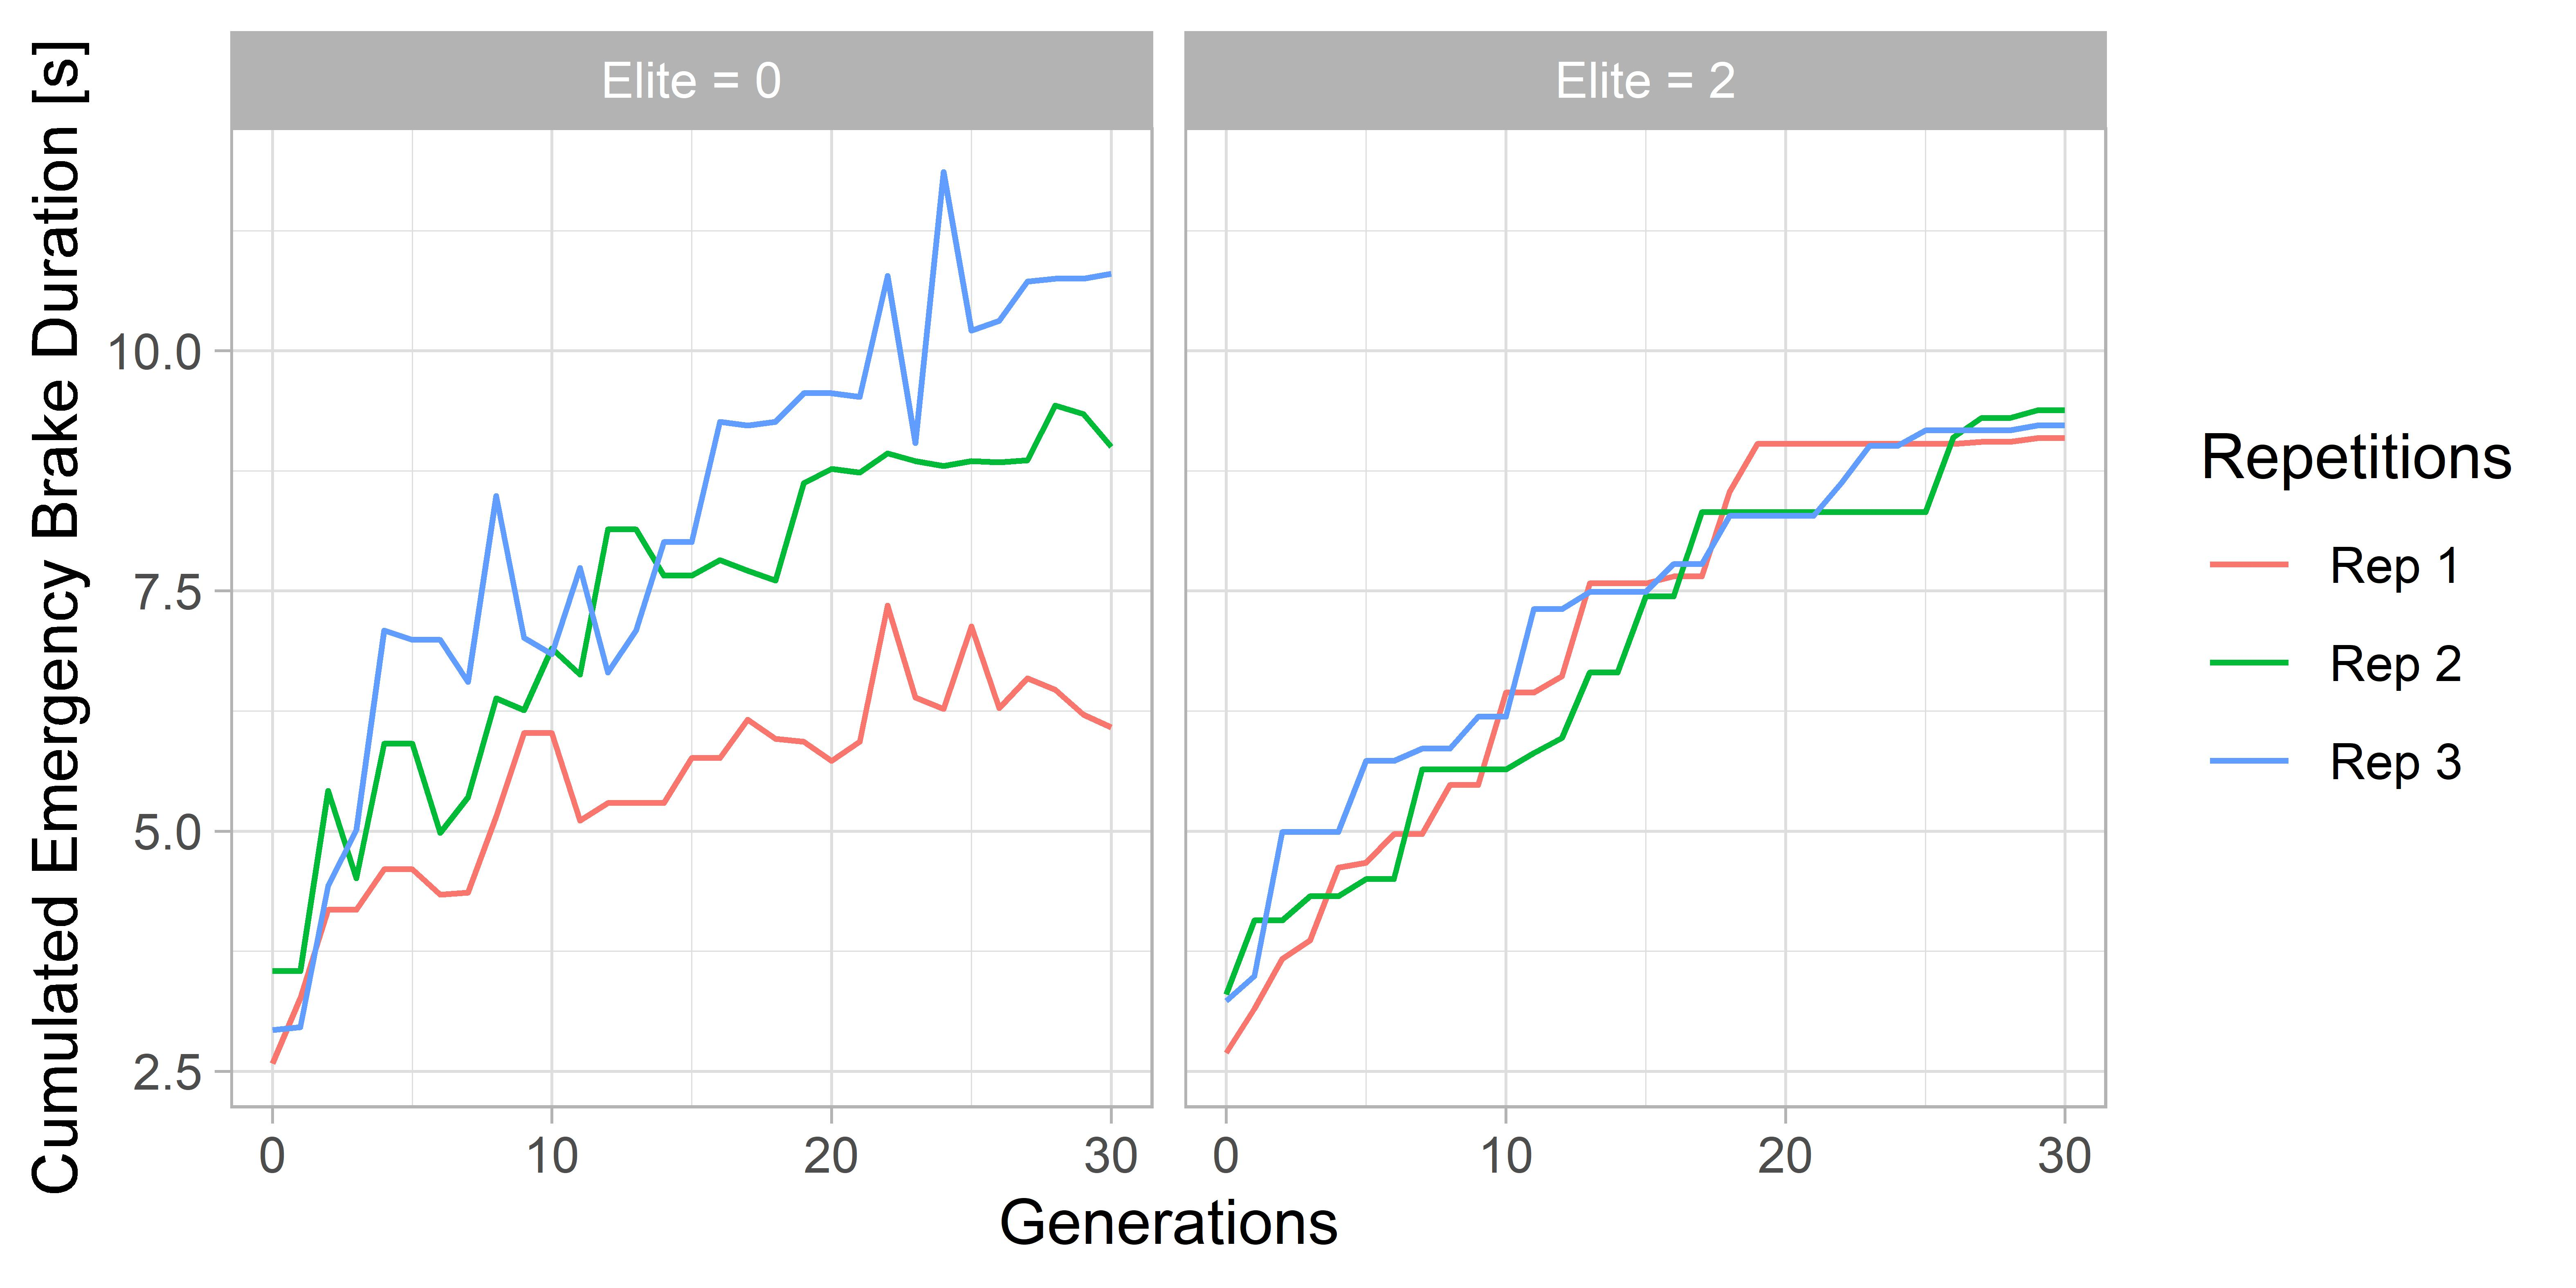
\includegraphics[width=1\linewidth]{simulations/evaluation/plots/elite_vs_no_elite_generations}
	\caption{elite selection comparison over GA generations}
	\label{fig:hyperparameter_tuning:elite_no_elite_comp}
\end{figure}

For analysing the statistical significance in the differences in mean between a genetic algorithm using elite selection of 2 vs no elite selection, a t-test can be used. To account for possible violation of the assumption of homogeneity, a robust welch's t-test is applied, which adjusts the DOF accordingly~\cite{field_discovering_2012}. On average, using elite improved the performance (M = 8.52, SE = 0.31), compared to using no elite (M = 7.92, SE = 0.55). This difference was not significant \textit{t}(14.21) = 0.96, p > 0.05; however, it did represent a small-sized effect r = 0.25. A visual comparison of both GAs, each repeated 10 times, can be seen in Figure \ref{fig:hyperparameter_tuning:elite_comparison}. Due to the existence of the aforementioned small effect as well as the reduced variance, it is concluded that elite selection of 2 is added to the settings from \ref{sect:hyperparameter_tuning:optimum_perf_caluclation}, which will be used in Chapter \ref{chap:evaluation}.

\begin{figure}[ht] 
	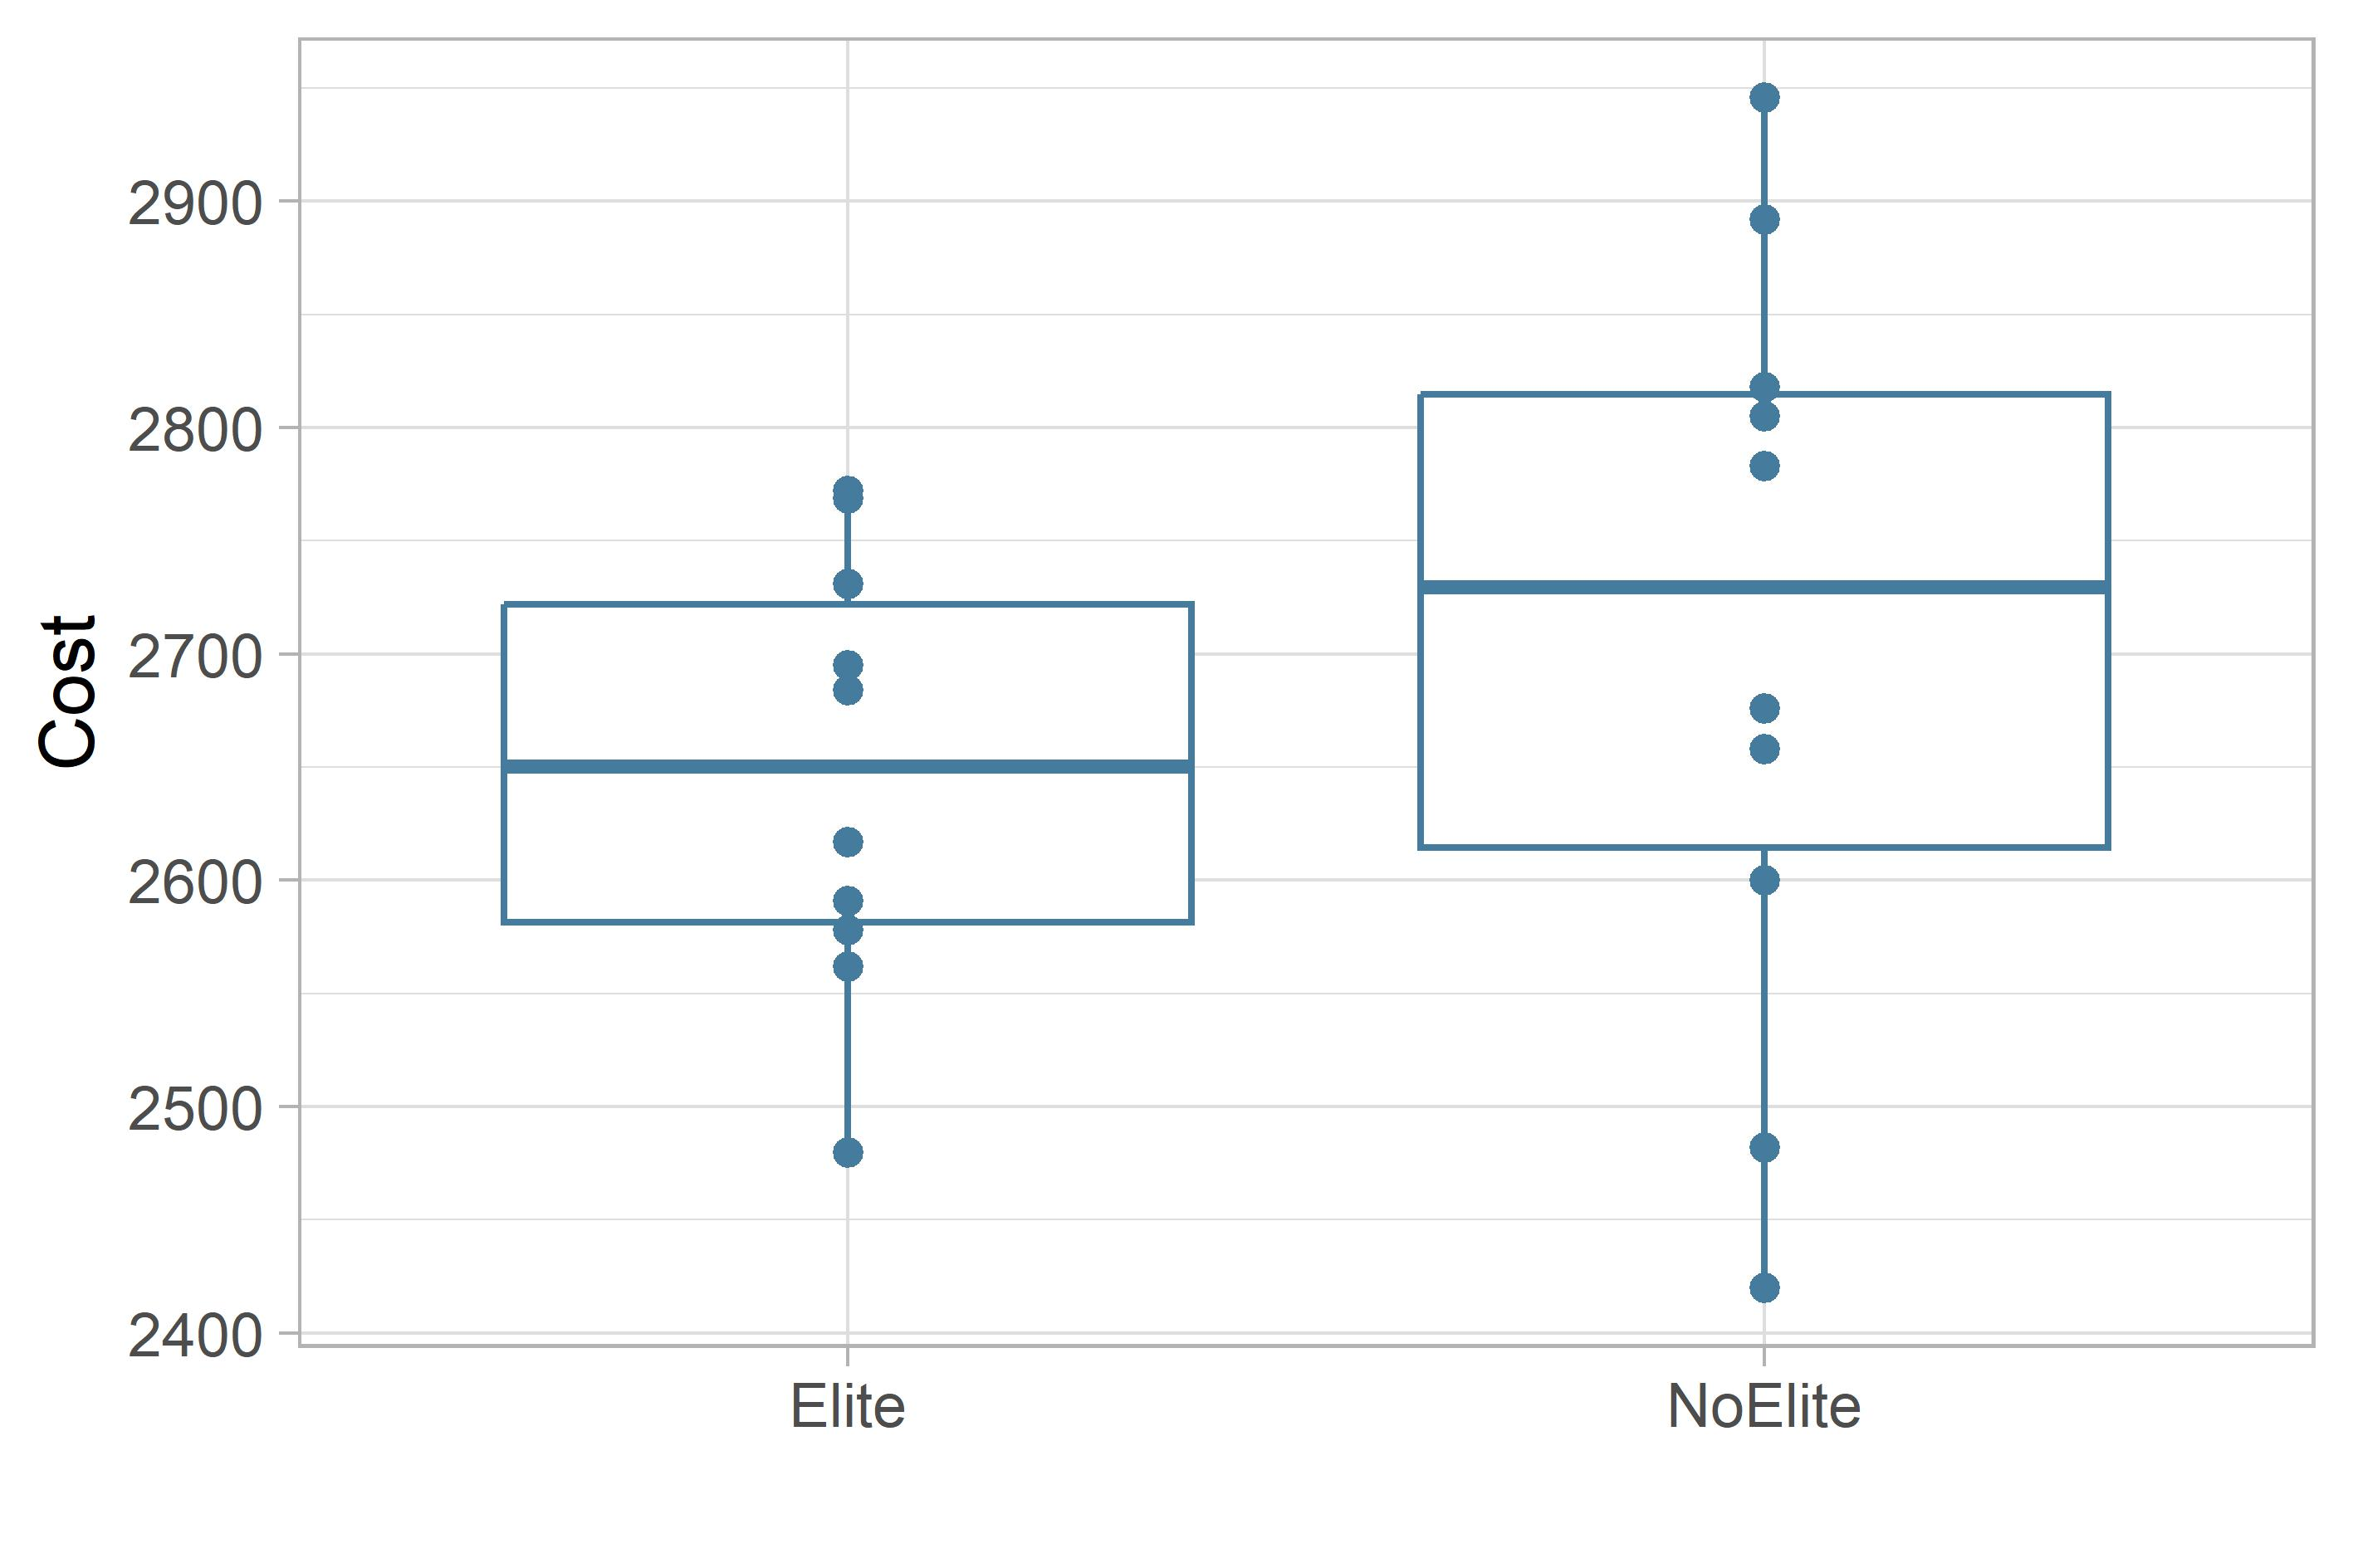
\includegraphics[width=1\linewidth]{simulations/evaluation/plots/elite_vs_no_elite}
	\caption{elite selection comparison results}
	\label{fig:hyperparameter_tuning:elite_comparison}
\end{figure}

\paragraph{Effect Size}
According to Field et al.~\cite{field_discovering_2012} effect sizes provide an objective measure on the importance of an effect, where 0 means no effect and 1 means a perfect effect. They allow for a standardized measure and are not affected by sample size. He further recommends to utilize the widely used suggestions made by Cohen~\cite{cohen_statistical_1988, cohen_power_1992} on defining between a large or small effect:

\begin{itemize}
	\item r = .10 (small effect): The effect explains 1\% of the variance. 
	\item r = .30 (medium effect): The effect explains 9\% of the variance. 
	\item r = .50 (large effect): The effect explains 25\% of the variance.
\end{itemize} 

Effect sizes also be used to compare different algorithms in Chapter \ref{chap:evaluation} as well and are calculated for a t-test using Equation \ref{equ:hyperparameter_tuning:effect_size}.

\begin{equation}
	\begin{split}
		r & = \sqrt{\frac{t^2}{t^2 + DOF}}
	\end{split}
	 \label{equ:hyperparameter_tuning:effect_size}
\end{equation}




